\documentclass[twoside]{book}

% Packages required by doxygen
\usepackage{calc}
\usepackage{doxygen}
\usepackage{graphicx}
\usepackage[utf8]{inputenc}
\usepackage{makeidx}
\usepackage{multicol}
\usepackage{multirow}
\usepackage{textcomp}
\usepackage[table]{xcolor}

% Font selection
\usepackage[T1]{fontenc}
\usepackage{mathptmx}
\usepackage[scaled=.90]{helvet}
\usepackage{courier}
\usepackage{amssymb}
\usepackage{sectsty}
\renewcommand{\familydefault}{\sfdefault}
\allsectionsfont{%
  \fontseries{bc}\selectfont%
  \color{darkgray}%
}
\renewcommand{\DoxyLabelFont}{%
  \fontseries{bc}\selectfont%
  \color{darkgray}%
}

% Page & text layout
\usepackage{geometry}
\geometry{%
  a4paper,%
  top=2.5cm,%
  bottom=2.5cm,%
  left=2.5cm,%
  right=2.5cm%
}
\tolerance=750
\hfuzz=15pt
\hbadness=750
\setlength{\emergencystretch}{15pt}
\setlength{\parindent}{0cm}
\setlength{\parskip}{0.2cm}
\makeatletter
\renewcommand{\paragraph}{%
  \@startsection{paragraph}{4}{0ex}{-1.0ex}{1.0ex}{%
    \normalfont\normalsize\bfseries\SS@parafont%
  }%
}
\renewcommand{\subparagraph}{%
  \@startsection{subparagraph}{5}{0ex}{-1.0ex}{1.0ex}{%
    \normalfont\normalsize\bfseries\SS@subparafont%
  }%
}
\makeatother

% Headers & footers
\usepackage{fancyhdr}
\pagestyle{fancyplain}
\fancyhead[LE]{\fancyplain{}{\bfseries\thepage}}
\fancyhead[CE]{\fancyplain{}{}}
\fancyhead[RE]{\fancyplain{}{\bfseries\leftmark}}
\fancyhead[LO]{\fancyplain{}{\bfseries\rightmark}}
\fancyhead[CO]{\fancyplain{}{}}
\fancyhead[RO]{\fancyplain{}{\bfseries\thepage}}
\fancyfoot[LE]{\fancyplain{}{}}
\fancyfoot[CE]{\fancyplain{}{}}
\fancyfoot[RE]{\fancyplain{}{\bfseries\scriptsize Generated on Mon Nov 29 2021 21\-:55\-:00 for Pa\-R\-L\-Schedv1.\-0 by Doxygen }}
\fancyfoot[LO]{\fancyplain{}{\bfseries\scriptsize Generated on Mon Nov 29 2021 21\-:55\-:00 for Pa\-R\-L\-Schedv1.\-0 by Doxygen }}
\fancyfoot[CO]{\fancyplain{}{}}
\fancyfoot[RO]{\fancyplain{}{}}
\renewcommand{\footrulewidth}{0.4pt}
\renewcommand{\chaptermark}[1]{%
  \markboth{#1}{}%
}
\renewcommand{\sectionmark}[1]{%
  \markright{\thesection\ #1}%
}

% Indices & bibliography
\usepackage{natbib}
\usepackage[titles]{tocloft}
\setcounter{tocdepth}{3}
\setcounter{secnumdepth}{5}
\makeindex

% Hyperlinks (required, but should be loaded last)
\usepackage{ifpdf}
\ifpdf
  \usepackage[pdftex,pagebackref=true]{hyperref}
\else
  \usepackage[ps2pdf,pagebackref=true]{hyperref}
\fi
\hypersetup{%
  colorlinks=true,%
  linkcolor=blue,%
  citecolor=blue,%
  unicode%
}

% Custom commands
\newcommand{\clearemptydoublepage}{%
  \newpage{\pagestyle{empty}\cleardoublepage}%
}


%===== C O N T E N T S =====

\begin{document}

% Titlepage & ToC
\hypersetup{pageanchor=false}
\pagenumbering{roman}
\begin{titlepage}
\vspace*{7cm}
\begin{center}%
{\Large Pa\-R\-L\-Schedv1.0 }\\
\vspace*{1cm}
{\large Generated by Doxygen 1.8.6}\\
\vspace*{0.5cm}
{\small Mon Nov 29 2021 21:55:00}\\
\end{center}
\end{titlepage}
\clearemptydoublepage
\tableofcontents
\clearemptydoublepage
\pagenumbering{arabic}
\hypersetup{pageanchor=true}

%--- Begin generated contents ---
\chapter{Class Index}
\section{Class List}
Here are the classes, structs, unions and interfaces with brief descriptions\-:\begin{DoxyCompactList}
\item\contentsline{section}{\hyperlink{structOptionData__}{Option\-Data\-\_\-} }{\pageref{structOptionData__}}{}
\end{DoxyCompactList}

\chapter{Class Documentation}
\hypertarget{structPerformance}{\section{Performance Struct Reference}
\label{structPerformance}\index{Performance@{Performance}}
}


{\ttfamily \#include $<$Performance\-Counters.\-h$>$}

\subsection*{Public Member Functions}
\begin{DoxyCompactItemize}
\item 
\hypertarget{structPerformance_a487d0bd5f7e07e516faf16def16d847f}{void {\bfseries reset} (void)}\label{structPerformance_a487d0bd5f7e07e516faf16def16d847f}

\end{DoxyCompactItemize}
\subsection*{Public Attributes}
\begin{DoxyCompactItemize}
\item 
\hypertarget{structPerformance_a46b912e5250284e086eae918593ea80d}{int {\bfseries num\-\_\-performance\-\_\-counters}}\label{structPerformance_a46b912e5250284e086eae918593ea80d}

\item 
\hypertarget{structPerformance_ae4f81f358bb251363fd30b1af212e587}{double {\bfseries initial\-\_\-tot\-\_\-ins}}\label{structPerformance_ae4f81f358bb251363fd30b1af212e587}

\item 
\hypertarget{structPerformance_aba1f3bc10aae0d5ee9294b79fbef41c9}{double {\bfseries initial\-\_\-tot\-\_\-cyc}}\label{structPerformance_aba1f3bc10aae0d5ee9294b79fbef41c9}

\item 
\hypertarget{structPerformance_aa22796680433fbf6ea9e7c0b3671e2bc}{double {\bfseries initial\-\_\-lst\-\_\-ins}}\label{structPerformance_aa22796680433fbf6ea9e7c0b3671e2bc}

\item 
\hypertarget{structPerformance_a47d5e630cab47e7db419244884b6c67c}{double {\bfseries initial\-\_\-\-L1misses}}\label{structPerformance_a47d5e630cab47e7db419244884b6c67c}

\item 
\hypertarget{structPerformance_abaa76cc9c0565e882f39ce7e67280c60}{double {\bfseries initial\-\_\-tlb\-\_\-dm}}\label{structPerformance_abaa76cc9c0565e882f39ce7e67280c60}

\item 
\hypertarget{structPerformance_a6ecd82d6779e5862c75ec9978fbcc507}{double {\bfseries time}}\label{structPerformance_a6ecd82d6779e5862c75ec9978fbcc507}

\end{DoxyCompactItemize}


\subsection{Detailed Description}
This structure captures different performance indicators of a thread 

Definition at line 23 of file Performance\-Counters.\-h.



The documentation for this struct was generated from the following file\-:\begin{DoxyCompactItemize}
\item 
Performance\-Counters.\-h\end{DoxyCompactItemize}

\hypertarget{classPerformanceCounters}{\section{Performance\-Counters Class Reference}
\label{classPerformanceCounters}\index{Performance\-Counters@{Performance\-Counters}}
}
\subsection*{Public Member Functions}
\begin{DoxyCompactItemize}
\item 
\hypertarget{classPerformanceCounters_a6da9d4ba5cdc2a27f12c134e3a536612}{int {\bfseries initialize} (void)}\label{classPerformanceCounters_a6da9d4ba5cdc2a27f12c134e3a536612}

\item 
\hypertarget{classPerformanceCounters_aaf18c08421469aa6f5cae87d6a1721dd}{void {\bfseries get\-\_\-performance} (\hyperlink{structPerformance}{Performance} \&performance)}\label{classPerformanceCounters_aaf18c08421469aa6f5cae87d6a1721dd}

\end{DoxyCompactItemize}


\subsection{Detailed Description}


Definition at line 43 of file Performance\-Counters.\-h.



The documentation for this class was generated from the following files\-:\begin{DoxyCompactItemize}
\item 
Performance\-Counters.\-h\item 
Performance\-Counters.\-cpp\end{DoxyCompactItemize}

\hypertarget{classScheduler}{\section{Scheduler Class Reference}
\label{classScheduler}\index{Scheduler@{Scheduler}}
}


{\ttfamily \#include $<$Scheduler.\-h$>$}

\subsection*{Public Member Functions}
\begin{DoxyCompactItemize}
\item 
\hyperlink{classScheduler_a9d9fdac53788885928fa849892250819}{Scheduler} (const std\-::string \&in\-\_\-file, const unsigned int \&num\-\_\-threads)
\item 
\hypertarget{classScheduler_aa55196b20c6a062b2f479776738622fd}{{\bfseries Scheduler} (const \hyperlink{classScheduler}{Scheduler} \&other)}\label{classScheduler_aa55196b20c6a062b2f479776738622fd}

\item 
\hypertarget{classScheduler_a8a41677eaa1266ec0ab41dcf0ac0d865}{\hyperlink{classScheduler}{Scheduler} \& {\bfseries operator=} (const \hyperlink{classScheduler}{Scheduler} \&other)}\label{classScheduler_a8a41677eaa1266ec0ab41dcf0ac0d865}

\item 
void \hyperlink{classScheduler_a27e2a247cde3ad80ac25b9188a1e17ee}{initialize} (const unsigned int \&num\-\_\-threads, const bool \&R\-L\-\_\-active\-\_\-reshuffling, const bool \&R\-L\-\_\-performance\-\_\-reshuffling, const double \&step\-\_\-size, const double \&L\-A\-M\-B\-D\-A, const double \&sched\-\_\-period, const bool \&suspend\-\_\-threads, const bool \&printout\-\_\-strategies, const bool \&printout\-\_\-actions, const bool \&write\-\_\-to\-\_\-files, const bool \&write\-\_\-to\-\_\-files\-\_\-details, const double \&gamma, const bool \&O\-S\-\_\-mapping, const bool \&R\-L\-\_\-mapping, const bool \&P\-R\-\_\-mapping, const bool \&S\-T\-\_\-mapping, const bool \&optimize\-\_\-main\-\_\-resource)
\item 
void \hyperlink{classScheduler_ac0f68dd6a14fdf70dc964c67dc8d39b2}{update} (const unsigned int \&resource\-\_\-ind, std\-::vector$<$ bool $>$ \&update\-\_\-inds)
\item 
void \hyperlink{classScheduler_a58fba108ce2748870a6288cd6f5fd1e3}{run} ()
\item 
void \hyperlink{classScheduler_ad187198f24a2b283a4628f0e0b3ffd84}{retrieve\-\_\-performances} (const unsigned int \&resource\-\_\-ind)
\item 
void \hyperlink{classScheduler_a2e8eeafda5ee215213d1a8ad076e86e7}{performance\-\_\-preprocessing} (const unsigned int \&resource\-\_\-ind)
\item 
void \hyperlink{classScheduler_a782dd674fc65f8f96bbcdad24e48b75e}{apply\-\_\-scheduling\-\_\-policy} ()
\item 
\hyperlink{structthread__info}{thread\-\_\-info} $\ast$ \hyperlink{classScheduler_a9e0189d3b9815eac90901ba171722525}{get\-\_\-tinfo} (void)
\item 
const unsigned int \& \hyperlink{classScheduler_ab640e06ed98152a9acd8cf032b7ad455}{get\-\_\-number\-\_\-threads} (void) const 
\end{DoxyCompactItemize}
\subsection*{Static Public Member Functions}
\begin{DoxyCompactItemize}
\item 
\hypertarget{classScheduler_adc23bd3b2f1babde08ce237c8f43cc19}{static void $\ast$ {\bfseries send\-\_\-wrapper} (void $\ast$object)}\label{classScheduler_adc23bd3b2f1babde08ce237c8f43cc19}

\end{DoxyCompactItemize}
\subsection*{Public Attributes}
\begin{DoxyCompactItemize}
\item 
\hypertarget{classScheduler_a991ae0f798df9ce56116d5c66f615c9f}{unsigned int {\bfseries counter\-\_\-of\-\_\-threads\-\_\-}}\label{classScheduler_a991ae0f798df9ce56116d5c66f615c9f}

\end{DoxyCompactItemize}


\subsection{Detailed Description}
\hyperlink{classScheduler}{Scheduler} 

Definition at line 36 of file Scheduler.\-h.



\subsection{Constructor \& Destructor Documentation}
\hypertarget{classScheduler_a9d9fdac53788885928fa849892250819}{\index{Scheduler@{Scheduler}!Scheduler@{Scheduler}}
\index{Scheduler@{Scheduler}!Scheduler@{Scheduler}}
\subsubsection[{Scheduler}]{\setlength{\rightskip}{0pt plus 5cm}Scheduler\-::\-Scheduler (
\begin{DoxyParamCaption}
\item[{const std\-::string \&}]{in\-\_\-file, }
\item[{const unsigned int \&}]{num\-\_\-threads}
\end{DoxyParamCaption}
)}}\label{classScheduler_a9d9fdac53788885928fa849892250819}
The first part defines the number of N\-U\-M\-A nodes that should be used for pinning

The first pair defines the number of C\-P\-U nodes that should be used for pinning from each N\-U\-M\-A node

N\-O\-N-\/\-A\-D\-J\-U\-S\-T\-A\-B\-L\-E P\-A\-R\-A\-M\-E\-T\-E\-R\-S (Please, do not change the following)

Definition at line 274 of file Scheduler.\-cpp.



\subsection{Member Function Documentation}
\hypertarget{classScheduler_a782dd674fc65f8f96bbcdad24e48b75e}{\index{Scheduler@{Scheduler}!apply\-\_\-scheduling\-\_\-policy@{apply\-\_\-scheduling\-\_\-policy}}
\index{apply\-\_\-scheduling\-\_\-policy@{apply\-\_\-scheduling\-\_\-policy}!Scheduler@{Scheduler}}
\subsubsection[{apply\-\_\-scheduling\-\_\-policy}]{\setlength{\rightskip}{0pt plus 5cm}void Scheduler\-::apply\-\_\-scheduling\-\_\-policy (
\begin{DoxyParamCaption}
{}
\end{DoxyParamCaption}
)}}\label{classScheduler_a782dd674fc65f8f96bbcdad24e48b75e}
Applying scheduling policy 

Definition at line 1535 of file Scheduler.\-cpp.



Referenced by run().

\hypertarget{classScheduler_ab640e06ed98152a9acd8cf032b7ad455}{\index{Scheduler@{Scheduler}!get\-\_\-number\-\_\-threads@{get\-\_\-number\-\_\-threads}}
\index{get\-\_\-number\-\_\-threads@{get\-\_\-number\-\_\-threads}!Scheduler@{Scheduler}}
\subsubsection[{get\-\_\-number\-\_\-threads}]{\setlength{\rightskip}{0pt plus 5cm}const unsigned int\& Scheduler\-::get\-\_\-number\-\_\-threads (
\begin{DoxyParamCaption}
\item[{void}]{}
\end{DoxyParamCaption}
) const\hspace{0.3cm}{\ttfamily [inline]}}}\label{classScheduler_ab640e06ed98152a9acd8cf032b7ad455}
Get number of threads \begin{DoxyReturn}{Returns}

\end{DoxyReturn}


Definition at line 139 of file Scheduler.\-h.

\hypertarget{classScheduler_a9e0189d3b9815eac90901ba171722525}{\index{Scheduler@{Scheduler}!get\-\_\-tinfo@{get\-\_\-tinfo}}
\index{get\-\_\-tinfo@{get\-\_\-tinfo}!Scheduler@{Scheduler}}
\subsubsection[{get\-\_\-tinfo}]{\setlength{\rightskip}{0pt plus 5cm}{\bf thread\-\_\-info}$\ast$ Scheduler\-::get\-\_\-tinfo (
\begin{DoxyParamCaption}
\item[{void}]{}
\end{DoxyParamCaption}
)\hspace{0.3cm}{\ttfamily [inline]}}}\label{classScheduler_a9e0189d3b9815eac90901ba171722525}
Get information of thread \begin{DoxyReturn}{Returns}

\end{DoxyReturn}


Definition at line 122 of file Scheduler.\-h.

\hypertarget{classScheduler_a27e2a247cde3ad80ac25b9188a1e17ee}{\index{Scheduler@{Scheduler}!initialize@{initialize}}
\index{initialize@{initialize}!Scheduler@{Scheduler}}
\subsubsection[{initialize}]{\setlength{\rightskip}{0pt plus 5cm}void Scheduler\-::initialize (
\begin{DoxyParamCaption}
\item[{const unsigned int \&}]{num\-\_\-threads, }
\item[{const bool \&}]{R\-L\-\_\-active\-\_\-reshuffling, }
\item[{const bool \&}]{R\-L\-\_\-performance\-\_\-reshuffling, }
\item[{const double \&}]{step\-\_\-size, }
\item[{const double \&}]{L\-A\-M\-B\-D\-A, }
\item[{const double \&}]{sched\-\_\-period, }
\item[{const bool \&}]{suspend\-\_\-threads, }
\item[{const bool \&}]{printout\-\_\-strategies, }
\item[{const bool \&}]{printout\-\_\-actions, }
\item[{const bool \&}]{write\-\_\-to\-\_\-files, }
\item[{const bool \&}]{write\-\_\-to\-\_\-files\-\_\-details, }
\item[{const double \&}]{gamma, }
\item[{const bool \&}]{O\-S\-\_\-mapping, }
\item[{const bool \&}]{R\-L\-\_\-mapping, }
\item[{const bool \&}]{P\-R\-\_\-mapping, }
\item[{const bool \&}]{S\-T\-\_\-mapping, }
\item[{const bool \&}]{optimize\-\_\-main\-\_\-resource}
\end{DoxyParamCaption}
)}}\label{classScheduler_a27e2a247cde3ad80ac25b9188a1e17ee}
Initialize \hyperlink{classScheduler}{Scheduler}


\begin{DoxyParams}{Parameters}
{\em num\-\_\-threads} & Number of threads \\
\hline
{\em R\-L\-\_\-active\-\_\-reshuffling} & Reshuffle R\-L strategies if active threads have changed \\
\hline
{\em R\-L\-\_\-performance\-\_\-reshuffling} & Reshuffle R\-L strategies if performance of active threads has dropped significantly \\
\hline
{\em step\-\_\-size} & Step size of R\-L algorithm \\
\hline
{\em L\-A\-M\-B\-D\-A} & Perturbation factor of R\-L algorithm \\
\hline
{\em sched\-\_\-period} & Scheduling period of the child resources \\
\hline
{\em suspend\-\_\-threads} & Suspend threads when switching N\-U\-M\-A nodes \\
\hline
{\em printout\-\_\-strategies} & \\
\hline
{\em printout\-\_\-actions} & \\
\hline
{\em write\-\_\-to\-\_\-files} & \\
\hline
{\em write\-\_\-to\-\_\-files\-\_\-details} & \\
\hline
{\em gamma} & Factor related to the definition of the balanced performance indicator \\
\hline
{\em O\-S\-\_\-mapping} & Mapping according to the O\-S scheduler \\
\hline
{\em R\-L\-\_\-mapping} & Mapping according to the R\-L scheduler \\
\hline
{\em P\-R\-\_\-mapping} & Mapping according to a predefined map \\
\hline
{\em S\-T\-\_\-mapping} & Perform also allocation of thread memory \\
\hline
{\em optimize\-\_\-main\-\_\-resource} & Optimize the use of N\-U\-M\-A nodes \\
\hline
\end{DoxyParams}
\hypertarget{classScheduler_a2e8eeafda5ee215213d1a8ad076e86e7}{\index{Scheduler@{Scheduler}!performance\-\_\-preprocessing@{performance\-\_\-preprocessing}}
\index{performance\-\_\-preprocessing@{performance\-\_\-preprocessing}!Scheduler@{Scheduler}}
\subsubsection[{performance\-\_\-preprocessing}]{\setlength{\rightskip}{0pt plus 5cm}void Scheduler\-::performance\-\_\-preprocessing (
\begin{DoxyParamCaption}
\item[{const unsigned int \&}]{resource\-\_\-ind}
\end{DoxyParamCaption}
)}}\label{classScheduler_a2e8eeafda5ee215213d1a8ad076e86e7}
Preprocessing of performances 
\begin{DoxyParams}{Parameters}
{\em resource\-\_\-ind} & \\
\hline
\end{DoxyParams}


Definition at line 1364 of file Scheduler.\-cpp.



References Struct\-\_\-\-Overall\-Performance\-::update\-\_\-ave\-\_\-balanced\-\_\-performance\-\_\-per\-\_\-main\-\_\-resource(), Struct\-\_\-\-Overall\-Performance\-::update\-\_\-ave\-\_\-balanced\-\_\-performances\-\_\-per\-\_\-main\-\_\-resource\-\_\-per\-\_\-action(), Struct\-\_\-\-Overall\-Performance\-::update\-\_\-ave\-\_\-performance\-\_\-per\-\_\-main\-\_\-resource(), Struct\-\_\-\-Overall\-Performance\-::update\-\_\-num\-\_\-threads\-\_\-using\-\_\-main\-\_\-resource\-\_\-per\-\_\-action(), Struct\-\_\-\-Overall\-Performance\-::update\-\_\-run\-\_\-average\-\_\-balanced\-\_\-performance\-\_\-per\-\_\-main\-\_\-resource(), Struct\-\_\-\-Overall\-Performance\-::update\-\_\-run\-\_\-average\-\_\-balanced\-\_\-performances\-\_\-per\-\_\-main\-\_\-resource\-\_\-per\-\_\-action(), Struct\-\_\-\-Overall\-Performance\-::update\-\_\-run\-\_\-average\-\_\-performance\-\_\-per\-\_\-main\-\_\-resource(), Struct\-\_\-\-Overall\-Performance\-::update\-\_\-sum\-\_\-balanced\-\_\-performances\-\_\-per\-\_\-main\-\_\-resource(), Struct\-\_\-\-Overall\-Performance\-::update\-\_\-sum\-\_\-balanced\-\_\-performances\-\_\-per\-\_\-main\-\_\-resource\-\_\-per\-\_\-action(), and Struct\-\_\-\-Overall\-Performance\-::update\-\_\-sum\-\_\-performances\-\_\-per\-\_\-main\-\_\-resource().



Referenced by run().



Here is the call graph for this function\-:\nopagebreak
\begin{figure}[H]
\begin{center}
\leavevmode
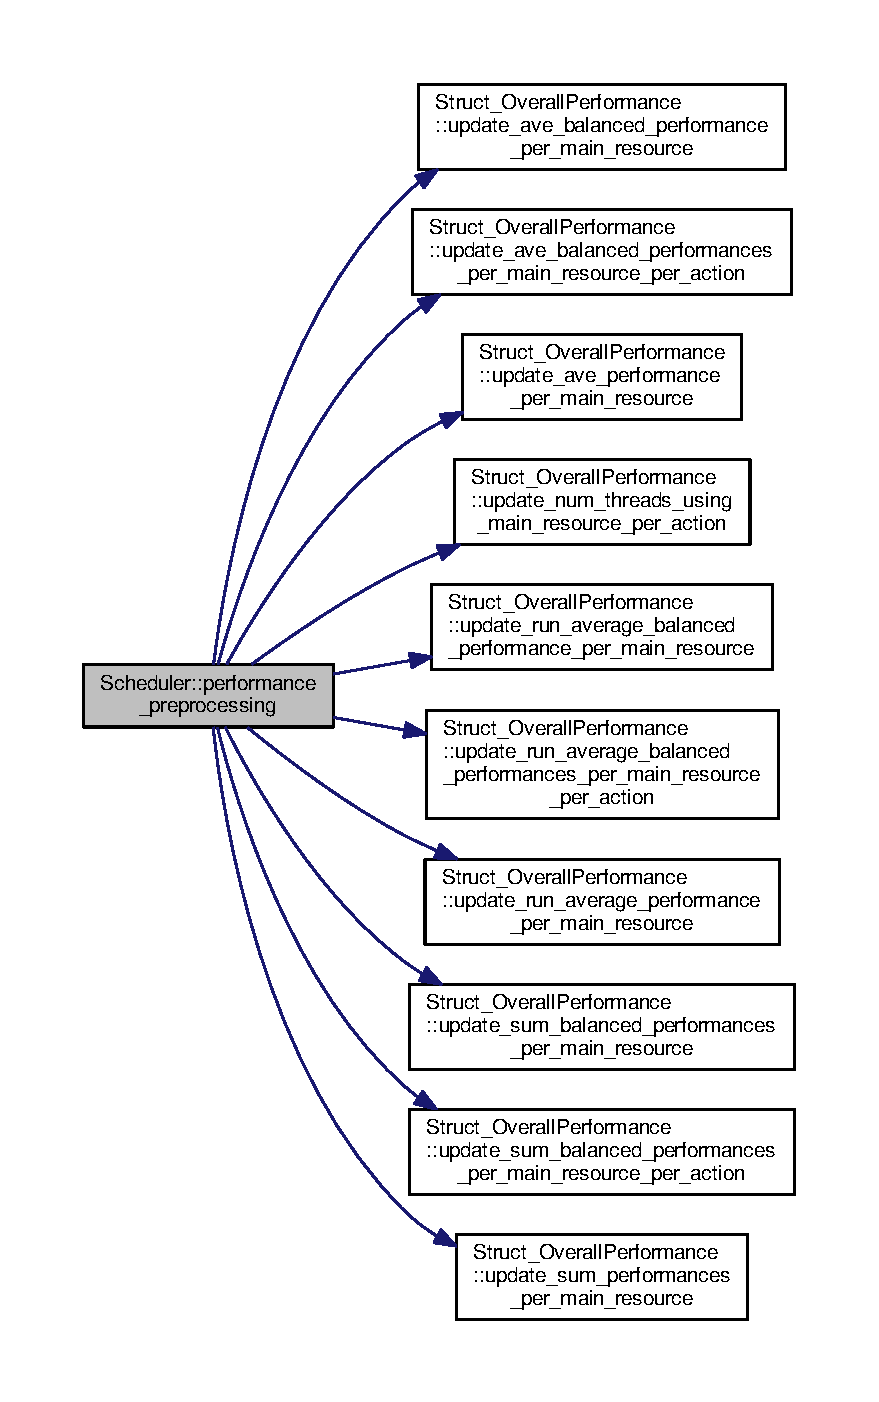
\includegraphics[height=550pt]{classScheduler_a2e8eeafda5ee215213d1a8ad076e86e7_cgraph}
\end{center}
\end{figure}


\hypertarget{classScheduler_ad187198f24a2b283a4628f0e0b3ffd84}{\index{Scheduler@{Scheduler}!retrieve\-\_\-performances@{retrieve\-\_\-performances}}
\index{retrieve\-\_\-performances@{retrieve\-\_\-performances}!Scheduler@{Scheduler}}
\subsubsection[{retrieve\-\_\-performances}]{\setlength{\rightskip}{0pt plus 5cm}void Scheduler\-::retrieve\-\_\-performances (
\begin{DoxyParamCaption}
\item[{const unsigned int \&}]{resource\-\_\-ind}
\end{DoxyParamCaption}
)}}\label{classScheduler_ad187198f24a2b283a4628f0e0b3ffd84}
Retrieve performances


\begin{DoxyParams}{Parameters}
{\em resource\-\_\-ind} & \\
\hline
\end{DoxyParams}


Definition at line 1298 of file Scheduler.\-cpp.



References Thread\-Control\-::thd\-\_\-record\-\_\-counters().



Referenced by run().



Here is the call graph for this function\-:\nopagebreak
\begin{figure}[H]
\begin{center}
\leavevmode
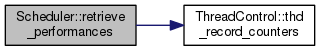
\includegraphics[width=312pt]{classScheduler_ad187198f24a2b283a4628f0e0b3ffd84_cgraph}
\end{center}
\end{figure}


\hypertarget{classScheduler_a58fba108ce2748870a6288cd6f5fd1e3}{\index{Scheduler@{Scheduler}!run@{run}}
\index{run@{run}!Scheduler@{Scheduler}}
\subsubsection[{run}]{\setlength{\rightskip}{0pt plus 5cm}void Scheduler\-::run (
\begin{DoxyParamCaption}
{}
\end{DoxyParamCaption}
)}}\label{classScheduler_a58fba108ce2748870a6288cd6f5fd1e3}
Run scheduler


\begin{DoxyParams}{Parameters}
{\em num\-\_\-threads} & \\
\hline
{\em rl\-\_\-mapping} & N\-O\-N-\/\-A\-D\-J\-U\-S\-T\-A\-B\-L\-E P\-A\-R\-A\-M\-E\-T\-E\-R\-S (Please, do not change the following) Parameters w.\-r.\-t. the R\-L\-\_\-mapping algorithm \\
\hline
\end{DoxyParams}


Definition at line 856 of file Scheduler.\-cpp.



References apply\-\_\-scheduling\-\_\-policy(), performance\-\_\-preprocessing(), retrieve\-\_\-performances(), and update().



Here is the call graph for this function\-:\nopagebreak
\begin{figure}[H]
\begin{center}
\leavevmode
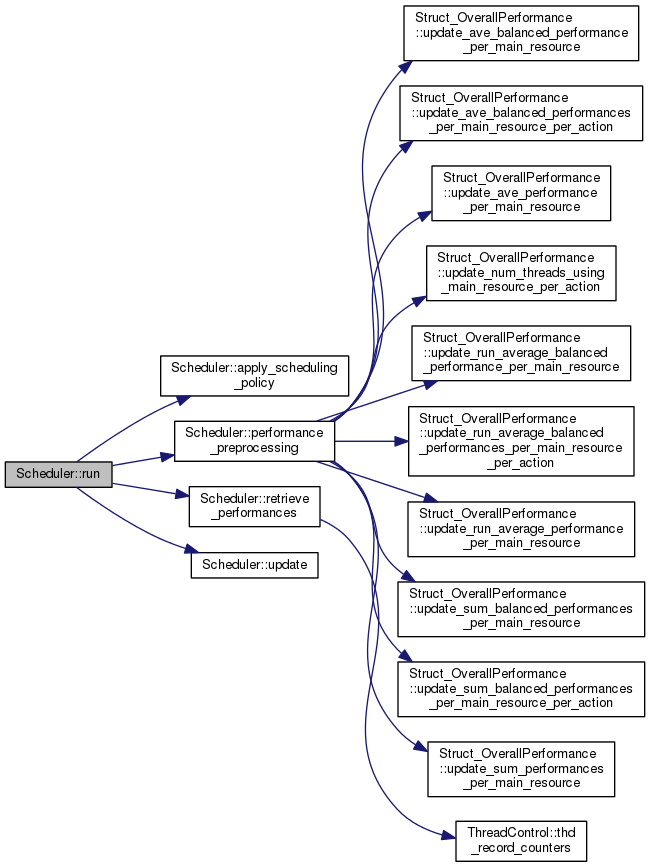
\includegraphics[width=350pt]{classScheduler_a58fba108ce2748870a6288cd6f5fd1e3_cgraph}
\end{center}
\end{figure}


\hypertarget{classScheduler_ac0f68dd6a14fdf70dc964c67dc8d39b2}{\index{Scheduler@{Scheduler}!update@{update}}
\index{update@{update}!Scheduler@{Scheduler}}
\subsubsection[{update}]{\setlength{\rightskip}{0pt plus 5cm}void Scheduler\-::update (
\begin{DoxyParamCaption}
\item[{const unsigned int \&}]{resource\-\_\-ind, }
\item[{std\-::vector$<$ bool $>$ \&}]{update\-\_\-inds}
\end{DoxyParamCaption}
)}}\label{classScheduler_ac0f68dd6a14fdf70dc964c67dc8d39b2}
Update scheduling decisions 
\begin{DoxyParams}{Parameters}
{\em resource\-\_\-ind} & \\
\hline
{\em update\-\_\-inds} & \\
\hline
\end{DoxyParams}


Definition at line 924 of file Scheduler.\-cpp.



Referenced by run().



The documentation for this class was generated from the following files\-:\begin{DoxyCompactItemize}
\item 
Scheduler.\-h\item 
Scheduler.\-cpp\end{DoxyCompactItemize}

\hypertarget{structStruct__Actions}{\section{Struct\-\_\-\-Actions Struct Reference}
\label{structStruct__Actions}\index{Struct\-\_\-\-Actions@{Struct\-\_\-\-Actions}}
}
\subsection*{Public Member Functions}
\begin{DoxyCompactItemize}
\item 
\hypertarget{structStruct__Actions_ad28379afcba301fca72e1e6939fa4c4f}{void {\bfseries initialize} (const std\-::string \&resource, const unsigned int \&num\-\_\-sources, const unsigned int \&max\-\_\-num\-\_\-sources\-\_\-user, std\-::vector$<$ unsigned int $>$ \&action\-\_\-main\-\_\-old, const unsigned int \&thread\-\_\-num)}\label{structStruct__Actions_ad28379afcba301fca72e1e6939fa4c4f}

\item 
\hypertarget{structStruct__Actions_a65aec6da3f4aa08047e285566fe45487}{void {\bfseries initialize\-\_\-w\-\_\-child} (const std\-::string \&resource, const unsigned int \&num\-\_\-sources, const unsigned int \&max\-\_\-num\-\_\-sources\-\_\-user, const std\-::string \&child\-\_\-resource, const std\-::vector$<$ std\-::vector$<$ unsigned int $>$ $>$ \&vec\-\_\-num\-\_\-child\-\_\-sources, const std\-::vector$<$ unsigned int $>$ \&vec\-\_\-max\-\_\-num\-\_\-child\-\_\-sources\-\_\-user, const unsigned int \&thread\-\_\-num, std\-::vector$<$ unsigned int $>$ \&action\-\_\-main\-\_\-old, const unsigned int \&policy, const unsigned int \&neighborhood\-\_\-size)}\label{structStruct__Actions_a65aec6da3f4aa08047e285566fe45487}

\item 
\hypertarget{structStruct__Actions_a2d1d697fe7778e807179b7bef8c809db}{std\-::vector$<$ unsigned int $>$ {\bfseries compute\-\_\-initial\-\_\-action} (const std\-::vector$<$ std\-::vector$<$ unsigned int $>$ $>$ \&vec\-\_\-num\-\_\-child\-\_\-sources, const std\-::vector$<$ unsigned int $>$ \&vec\-\_\-max\-\_\-num\-\_\-child\-\_\-sources\-\_\-user, const unsigned int \&thread\-\_\-num, const unsigned int \&max\-\_\-number\-\_\-available\-\_\-main\-\_\-sources)}\label{structStruct__Actions_a2d1d697fe7778e807179b7bef8c809db}

\item 
\hypertarget{structStruct__Actions_a41346a1cddc836c0fcf0509debb5bcd6}{std\-::vector$<$ unsigned int $>$ {\bfseries compute\-\_\-initial\-\_\-action\-\_\-rr} (const std\-::vector$<$ std\-::vector$<$ unsigned int $>$ $>$ \&vec\-\_\-num\-\_\-child\-\_\-sources, const std\-::vector$<$ unsigned int $>$ \&vec\-\_\-max\-\_\-num\-\_\-child\-\_\-sources\-\_\-user, const unsigned int \&thread\-\_\-num)}\label{structStruct__Actions_a41346a1cddc836c0fcf0509debb5bcd6}

\end{DoxyCompactItemize}
\subsection*{Public Attributes}
\begin{DoxyCompactItemize}
\item 
\hypertarget{structStruct__Actions_ac929169603c419d6a0d1e6cb8dacc980}{std\-::string {\bfseries resource\-\_\-}}\label{structStruct__Actions_ac929169603c419d6a0d1e6cb8dacc980}

\item 
\hypertarget{structStruct__Actions_aa3d36d82f026212fb1f59dac88da98b2}{std\-::string {\bfseries child\-\_\-resource\-\_\-}}\label{structStruct__Actions_aa3d36d82f026212fb1f59dac88da98b2}

\item 
\hypertarget{structStruct__Actions_a5042128cbd5fb915614f1309ad1b2cf2}{unsigned int {\bfseries num\-\_\-actions\-\_\-main\-\_\-resource\-\_\-}}\label{structStruct__Actions_a5042128cbd5fb915614f1309ad1b2cf2}

\item 
\hypertarget{structStruct__Actions_a7e5104b8c833631f55201f20433680f4}{std\-::vector$<$ unsigned int $>$ {\bfseries vec\-\_\-num\-\_\-child\-\_\-actions\-\_\-per\-\_\-main\-\_\-resource\-\_\-}}\label{structStruct__Actions_a7e5104b8c833631f55201f20433680f4}

\item 
\hypertarget{structStruct__Actions_ae03ee4c360ea92bd7c381d113047c11f}{std\-::map$<$ std\-::tuple$<$ unsigned \\*
int, unsigned int, unsigned \\*
int $>$, std\-::vector$<$ unsigned \\*
int $>$ $>$ {\bfseries map\-\_\-neighbors\-\_\-}}\label{structStruct__Actions_ae03ee4c360ea92bd7c381d113047c11f}

\item 
\hypertarget{structStruct__Actions_a687f670fd743b3c4ae86daf8cf2be3b4}{unsigned int {\bfseries action\-\_\-per\-\_\-main\-\_\-source\-\_\-}}\label{structStruct__Actions_a687f670fd743b3c4ae86daf8cf2be3b4}

\item 
\hypertarget{structStruct__Actions_a500af033d64e40e926d47ca3abb69397}{unsigned int {\bfseries previous\-\_\-action\-\_\-per\-\_\-main\-\_\-source\-\_\-}}\label{structStruct__Actions_a500af033d64e40e926d47ca3abb69397}

\item 
\hypertarget{structStruct__Actions_a58e3c004e83fe50762c69d6d4bc50022}{unsigned int {\bfseries action\-\_\-per\-\_\-child\-\_\-source\-\_\-}}\label{structStruct__Actions_a58e3c004e83fe50762c69d6d4bc50022}

\item 
\hypertarget{structStruct__Actions_abf351c2b735511e15a54c3821002b9da}{unsigned int {\bfseries previous\-\_\-action\-\_\-per\-\_\-child\-\_\-source\-\_\-}}\label{structStruct__Actions_abf351c2b735511e15a54c3821002b9da}

\item 
\hypertarget{structStruct__Actions_aae321f0f30f1249a87113e4dd9644630}{std\-::vector$<$ std\-::vector\\*
$<$ unsigned int $>$ $>$ {\bfseries vec\-\_\-child\-\_\-sources\-\_\-}}\label{structStruct__Actions_aae321f0f30f1249a87113e4dd9644630}

\end{DoxyCompactItemize}


\subsection{Detailed Description}


Definition at line 26 of file Methods\-Actions.\-h.



The documentation for this struct was generated from the following file\-:\begin{DoxyCompactItemize}
\item 
Methods\-Actions.\-h\end{DoxyCompactItemize}

\hypertarget{structStruct__Estimate}{\section{Struct\-\_\-\-Estimate Struct Reference}
\label{structStruct__Estimate}\index{Struct\-\_\-\-Estimate@{Struct\-\_\-\-Estimate}}
}


{\ttfamily \#include $<$Methods\-Estimate.\-h$>$}

\subsection*{Public Member Functions}
\begin{DoxyCompactItemize}
\item 
void \hyperlink{structStruct__Estimate_a86b258312b0cbd9a988a8b8c80f72fb4}{initialize} (const std\-::string \&resource, const unsigned int \&num\-\_\-sources, const unsigned int \&max\-\_\-num\-\_\-sources\-\_\-user, const unsigned int \&initial\-\_\-action, const bool \&mixed)
\item 
void \hyperlink{structStruct__Estimate_a14707ec3b60745fc143894f8b335e2eb}{initialize\-\_\-w\-\_\-child} (const std\-::string \&resource, const unsigned int \&num\-\_\-sources, const unsigned int \&max\-\_\-num\-\_\-sources\-\_\-user, const std\-::string \&child\-\_\-resource, const std\-::vector$<$ std\-::vector$<$ unsigned int $>$ $>$ \&vec\-\_\-num\-\_\-child\-\_\-sources, const std\-::vector$<$ unsigned int $>$ \&vec\-\_\-max\-\_\-num\-\_\-child\-\_\-sources\-\_\-user, const unsigned int \&thread\-\_\-num)
\item 
void \hyperlink{structStruct__Estimate_a1319536e0446f7017c1551375b7bd6bc}{update\-\_\-estimates} (const std\-::vector$<$ double $>$ \&vec\-\_\-estimates)
\item 
void \hyperlink{structStruct__Estimate_aafbf20ed9ca283b3d8e2da6a2d44a43e}{update\-\_\-child\-\_\-estimate} (const std\-::vector$<$ double $>$ \&vec\-\_\-estimates, const unsigned int \&source\-\_\-num)
\item 
void \hyperlink{structStruct__Estimate_a304683373750daa1d4409658ab5e3164}{update\-\_\-action} (const std\-::vector$<$ double $>$ \&vec\-\_\-estimates, const unsigned int \&source\-\_\-num)
\end{DoxyCompactItemize}
\subsection*{Public Attributes}
\begin{DoxyCompactItemize}
\item 
\hypertarget{structStruct__Estimate_a7866b20f273f4bbe7ce2645c5b434a35}{std\-::string {\bfseries resource\-\_\-}}\label{structStruct__Estimate_a7866b20f273f4bbe7ce2645c5b434a35}

\item 
\hypertarget{structStruct__Estimate_a24bdea270a40349a809470af81bafb0e}{unsigned int {\bfseries num\-\_\-sources\-\_\-}}\label{structStruct__Estimate_a24bdea270a40349a809470af81bafb0e}

\item 
\hypertarget{structStruct__Estimate_adabb78baf36f2ef0bc0d0e8e04828b97}{std\-::vector$<$ std\-::vector\\*
$<$ unsigned int $>$ $>$ {\bfseries vec\-\_\-child\-\_\-sources\-\_\-}}\label{structStruct__Estimate_adabb78baf36f2ef0bc0d0e8e04828b97}

\item 
\hypertarget{structStruct__Estimate_a0b0945a15f4acdd71673c1d1e45b567a}{std\-::vector$<$ double $>$ {\bfseries vec\-\_\-estimates\-\_\-}}\label{structStruct__Estimate_a0b0945a15f4acdd71673c1d1e45b567a}

\item 
\hypertarget{structStruct__Estimate_a897b46cd85b87c27a982bf18186c9f64}{std\-::vector$<$ double $>$ {\bfseries vec\-\_\-cummulative\-\_\-estimates\-\_\-}}\label{structStruct__Estimate_a897b46cd85b87c27a982bf18186c9f64}

\item 
\hypertarget{structStruct__Estimate_a85fe5ddb41f66097b960f2f715cc82c4}{double {\bfseries run\-\_\-average\-\_\-performance\-\_\-}}\label{structStruct__Estimate_a85fe5ddb41f66097b960f2f715cc82c4}

\item 
\hypertarget{structStruct__Estimate_a94dbf41446b7bad1f8c161c16e9f22c1}{std\-::vector$<$ \hyperlink{structStruct__Estimate}{Struct\-\_\-\-Estimate} $>$ {\bfseries vec\-\_\-child\-\_\-estimates\-\_\-}}\label{structStruct__Estimate_a94dbf41446b7bad1f8c161c16e9f22c1}

\item 
\hypertarget{structStruct__Estimate_a39eecaa17793e0813cdb89338ed794f3}{double {\bfseries low\-\_\-benchmark\-\_\-}}\label{structStruct__Estimate_a39eecaa17793e0813cdb89338ed794f3}

\item 
\hypertarget{structStruct__Estimate_aa876453ecd5a4e13ab9bf772ea4daac5}{double {\bfseries high\-\_\-benchmark\-\_\-}}\label{structStruct__Estimate_aa876453ecd5a4e13ab9bf772ea4daac5}

\item 
\hypertarget{structStruct__Estimate_a9fba7f1bb54a7b5a3f1683f2a567e3d7}{double {\bfseries maximum\-\_\-performance\-\_\-}}\label{structStruct__Estimate_a9fba7f1bb54a7b5a3f1683f2a567e3d7}

\item 
\hypertarget{structStruct__Estimate_aa1470fc0ef35f78f59abd0cc51916711}{bool {\bfseries random\-\_\-switch\-\_\-}}\label{structStruct__Estimate_aa1470fc0ef35f78f59abd0cc51916711}

\item 
\hypertarget{structStruct__Estimate_ac267b3a432bde596b9bf3548c7ac65df}{bool {\bfseries action\-\_\-change\-\_\-}}\label{structStruct__Estimate_ac267b3a432bde596b9bf3548c7ac65df}

\end{DoxyCompactItemize}


\subsection{Detailed Description}
\hyperlink{structStruct__Estimate}{Struct\-\_\-\-Estimate}

It provides the necessary information for keeping track our estimates for the performance of a thread over a specific node/cpu or the performance of a thread's memory over a specific node (or some further refinement if possible)

This structure is planned for 'per-\/thread' use, since it will hold estimates over the proper use of resources by each thread separately.

Within this structure, there is an additional struct that tracks the performances of the threads throughout the running time. 

Definition at line 43 of file Methods\-Estimate.\-h.



\subsection{Member Function Documentation}
\hypertarget{structStruct__Estimate_a86b258312b0cbd9a988a8b8c80f72fb4}{\index{Struct\-\_\-\-Estimate@{Struct\-\_\-\-Estimate}!initialize@{initialize}}
\index{initialize@{initialize}!Struct_Estimate@{Struct\-\_\-\-Estimate}}
\subsubsection[{initialize}]{\setlength{\rightskip}{0pt plus 5cm}void Struct\-\_\-\-Estimate\-::initialize (
\begin{DoxyParamCaption}
\item[{const std\-::string \&}]{resource, }
\item[{const unsigned int \&}]{num\-\_\-sources, }
\item[{const unsigned int \&}]{max\-\_\-num\-\_\-sources\-\_\-user, }
\item[{const unsigned int \&}]{initial\-\_\-action, }
\item[{const bool \&}]{mixed}
\end{DoxyParamCaption}
)\hspace{0.3cm}{\ttfamily [inline]}}}\label{structStruct__Estimate_a86b258312b0cbd9a988a8b8c80f72fb4}
This function initializes the structure


\begin{DoxyParams}{Parameters}
{\em resource} & resource type \\
\hline
{\em num\-\_\-sources} & number of sources \\
\hline
{\em max\-\_\-num\-\_\-sources\-\_\-user} & maximum number of sources per user \\
\hline
{\em initial\-\_\-action} & initial action \\
\hline
{\em mixed} & \\
\hline
\end{DoxyParams}


Definition at line 74 of file Methods\-Estimate.\-h.



Referenced by initialize\-\_\-w\-\_\-child().

\hypertarget{structStruct__Estimate_a14707ec3b60745fc143894f8b335e2eb}{\index{Struct\-\_\-\-Estimate@{Struct\-\_\-\-Estimate}!initialize\-\_\-w\-\_\-child@{initialize\-\_\-w\-\_\-child}}
\index{initialize\-\_\-w\-\_\-child@{initialize\-\_\-w\-\_\-child}!Struct_Estimate@{Struct\-\_\-\-Estimate}}
\subsubsection[{initialize\-\_\-w\-\_\-child}]{\setlength{\rightskip}{0pt plus 5cm}void Struct\-\_\-\-Estimate\-::initialize\-\_\-w\-\_\-child (
\begin{DoxyParamCaption}
\item[{const std\-::string \&}]{resource, }
\item[{const unsigned int \&}]{num\-\_\-sources, }
\item[{const unsigned int \&}]{max\-\_\-num\-\_\-sources\-\_\-user, }
\item[{const std\-::string \&}]{child\-\_\-resource, }
\item[{const std\-::vector$<$ std\-::vector$<$ unsigned int $>$ $>$ \&}]{vec\-\_\-num\-\_\-child\-\_\-sources, }
\item[{const std\-::vector$<$ unsigned int $>$ \&}]{vec\-\_\-max\-\_\-num\-\_\-child\-\_\-sources\-\_\-user, }
\item[{const unsigned int \&}]{thread\-\_\-num}
\end{DoxyParamCaption}
)\hspace{0.3cm}{\ttfamily [inline]}}}\label{structStruct__Estimate_a14707ec3b60745fc143894f8b335e2eb}
It is implicitly assumed that the main resource also has a child resource For example, in the case of P\-R\-O\-C\-E\-S\-S\-I\-N\-G\-\_\-\-B\-A\-N\-D\-W\-I\-D\-T\-H, the main sources correspond to the N\-U\-M\-A nodes (if available) while the child sources correspond to the C\-P\-U units available in each N\-U\-M\-A node.


\begin{DoxyParams}{Parameters}
{\em resource} & resource type \\
\hline
{\em num\-\_\-sources} & number of sources \\
\hline
{\em max\-\_\-num\-\_\-sources\-\_\-user} & maximum number of sources per user \\
\hline
{\em child\-\_\-resource} & child resource type \\
\hline
{\em vec\-\_\-num\-\_\-child\-\_\-sources} & vector of number of child sources \\
\hline
{\em vec\-\_\-max\-\_\-num\-\_\-child\-\_\-sources\-\_\-user} & vector of maximum number of child sources per user \\
\hline
{\em thread\-\_\-num} & thread number \\
\hline
\end{DoxyParams}


Definition at line 129 of file Methods\-Estimate.\-h.



References Struct\-\_\-\-Actions\-::compute\-\_\-initial\-\_\-action(), and initialize().



Here is the call graph for this function\-:\nopagebreak
\begin{figure}[H]
\begin{center}
\leavevmode
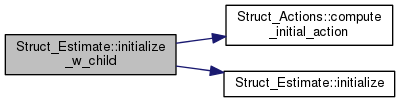
\includegraphics[width=350pt]{structStruct__Estimate_a14707ec3b60745fc143894f8b335e2eb_cgraph}
\end{center}
\end{figure}


\hypertarget{structStruct__Estimate_a304683373750daa1d4409658ab5e3164}{\index{Struct\-\_\-\-Estimate@{Struct\-\_\-\-Estimate}!update\-\_\-action@{update\-\_\-action}}
\index{update\-\_\-action@{update\-\_\-action}!Struct_Estimate@{Struct\-\_\-\-Estimate}}
\subsubsection[{update\-\_\-action}]{\setlength{\rightskip}{0pt plus 5cm}void Struct\-\_\-\-Estimate\-::update\-\_\-action (
\begin{DoxyParamCaption}
\item[{const std\-::vector$<$ double $>$ \&}]{vec\-\_\-estimates, }
\item[{const unsigned int \&}]{source\-\_\-num}
\end{DoxyParamCaption}
)\hspace{0.3cm}{\ttfamily [inline]}}}\label{structStruct__Estimate_a304683373750daa1d4409658ab5e3164}

\begin{DoxyParams}{Parameters}
{\em vec\-\_\-estimates} & \\
\hline
{\em source\-\_\-num} & \\
\hline
\end{DoxyParams}


Definition at line 225 of file Methods\-Estimate.\-h.

\hypertarget{structStruct__Estimate_aafbf20ed9ca283b3d8e2da6a2d44a43e}{\index{Struct\-\_\-\-Estimate@{Struct\-\_\-\-Estimate}!update\-\_\-child\-\_\-estimate@{update\-\_\-child\-\_\-estimate}}
\index{update\-\_\-child\-\_\-estimate@{update\-\_\-child\-\_\-estimate}!Struct_Estimate@{Struct\-\_\-\-Estimate}}
\subsubsection[{update\-\_\-child\-\_\-estimate}]{\setlength{\rightskip}{0pt plus 5cm}void Struct\-\_\-\-Estimate\-::update\-\_\-child\-\_\-estimate (
\begin{DoxyParamCaption}
\item[{const std\-::vector$<$ double $>$ \&}]{vec\-\_\-estimates, }
\item[{const unsigned int \&}]{source\-\_\-num}
\end{DoxyParamCaption}
)\hspace{0.3cm}{\ttfamily [inline]}}}\label{structStruct__Estimate_aafbf20ed9ca283b3d8e2da6a2d44a43e}
This function receives a vector of estimates for the child resources, and assigns it to the existing structure


\begin{DoxyParams}{Parameters}
{\em vec\-\_\-estimates} & \\
\hline
{\em source\-\_\-num} & \\
\hline
\end{DoxyParams}


Definition at line 213 of file Methods\-Estimate.\-h.

\hypertarget{structStruct__Estimate_a1319536e0446f7017c1551375b7bd6bc}{\index{Struct\-\_\-\-Estimate@{Struct\-\_\-\-Estimate}!update\-\_\-estimates@{update\-\_\-estimates}}
\index{update\-\_\-estimates@{update\-\_\-estimates}!Struct_Estimate@{Struct\-\_\-\-Estimate}}
\subsubsection[{update\-\_\-estimates}]{\setlength{\rightskip}{0pt plus 5cm}void Struct\-\_\-\-Estimate\-::update\-\_\-estimates (
\begin{DoxyParamCaption}
\item[{const std\-::vector$<$ double $>$ \&}]{vec\-\_\-estimates}
\end{DoxyParamCaption}
)\hspace{0.3cm}{\ttfamily [inline]}}}\label{structStruct__Estimate_a1319536e0446f7017c1551375b7bd6bc}
This function receives a vector of estimates, and assigns it to the existing structure


\begin{DoxyParams}{Parameters}
{\em vec\-\_\-estimates} & \\
\hline
\end{DoxyParams}


Definition at line 201 of file Methods\-Estimate.\-h.



The documentation for this struct was generated from the following file\-:\begin{DoxyCompactItemize}
\item 
Methods\-Estimate.\-h\end{DoxyCompactItemize}

\hypertarget{structStruct__MethodsEstimate}{\section{Struct\-\_\-\-Methods\-Estimate Struct Reference}
\label{structStruct__MethodsEstimate}\index{Struct\-\_\-\-Methods\-Estimate@{Struct\-\_\-\-Methods\-Estimate}}
}


{\ttfamily \#include $<$Methods\-Estimate.\-h$>$}

\subsection*{Public Member Functions}
\begin{DoxyCompactItemize}
\item 
void \hyperlink{structStruct__MethodsEstimate_a79b0089392ec35169c185f465f88b675}{R\-L\-\_\-update} (double \&maximum\-\_\-performance, std\-::vector$<$ double $>$ \&vec\-\_\-estimates, std\-::vector$<$ double $>$ \&vec\-\_\-cummulative\-\_\-estimates, const double \&current\-\_\-performance, const double \&current\-\_\-run\-\_\-ave\-\_\-performance, const unsigned int \&current\-\_\-action, const bool \&action\-\_\-main\-\_\-changed, const double \&step\-\_\-size\-\_\-\-R\-L, const bool \&R\-L\-\_\-active\-\_\-reshuffling, const bool \&R\-L\-\_\-performance\-\_\-reshuffling, const double \&factor\-\_\-h, const bool \&active\-\_\-threads\-\_\-change, const unsigned int \&thread)
\item 
\hypertarget{structStruct__MethodsEstimate_a13f8ba793252f8883a1769dbee5ddaaa}{void {\bfseries R\-L\-\_\-reshuffle\-\_\-mixed} (std\-::vector$<$ double $>$ \&vec\-\_\-estimates)}\label{structStruct__MethodsEstimate_a13f8ba793252f8883a1769dbee5ddaaa}

\item 
void \hyperlink{structStruct__MethodsEstimate_a81e63589cf2c8a3f83fbef1a16491aea}{A\-L\-\_\-update} (const double \&current\-\_\-performance, const double \&current\-\_\-run\-\_\-ave\-\_\-performance, const double \&run\-\_\-ave\-\_\-performance\-\_\-before, const double \&step\-\_\-size, const bool \&active\-\_\-threads\-\_\-change, const unsigned int \&thread, double \&low\-\_\-benchmark, double \&high\-\_\-benchmark, bool \&random\-\_\-switch, bool \&action\-\_\-change)
\end{DoxyCompactItemize}


\subsection{Detailed Description}
This structure provides alternative methodologies for creating estimates over the best selection. Inputs\-: For now, we assume that it takes as inputs the following\-:
\begin{DoxyItemize}
\item prior estimate data (maybe not created under the same rule)
\item current performance (this may take different values depending on the resource to be allocated) 
\end{DoxyItemize}

Definition at line 237 of file Methods\-Estimate.\-h.



\subsection{Member Function Documentation}
\hypertarget{structStruct__MethodsEstimate_a81e63589cf2c8a3f83fbef1a16491aea}{\index{Struct\-\_\-\-Methods\-Estimate@{Struct\-\_\-\-Methods\-Estimate}!A\-L\-\_\-update@{A\-L\-\_\-update}}
\index{A\-L\-\_\-update@{A\-L\-\_\-update}!Struct_MethodsEstimate@{Struct\-\_\-\-Methods\-Estimate}}
\subsubsection[{A\-L\-\_\-update}]{\setlength{\rightskip}{0pt plus 5cm}void Struct\-\_\-\-Methods\-Estimate\-::\-A\-L\-\_\-update (
\begin{DoxyParamCaption}
\item[{const double \&}]{current\-\_\-performance, }
\item[{const double \&}]{current\-\_\-run\-\_\-ave\-\_\-performance, }
\item[{const double \&}]{run\-\_\-ave\-\_\-performance\-\_\-before, }
\item[{const double \&}]{step\-\_\-size, }
\item[{const bool \&}]{active\-\_\-threads\-\_\-change, }
\item[{const unsigned int \&}]{thread, }
\item[{double \&}]{low\-\_\-benchmark, }
\item[{double \&}]{high\-\_\-benchmark, }
\item[{bool \&}]{random\-\_\-switch, }
\item[{bool \&}]{action\-\_\-change}
\end{DoxyParamCaption}
)\hspace{0.3cm}{\ttfamily [inline]}}}\label{structStruct__MethodsEstimate_a81e63589cf2c8a3f83fbef1a16491aea}
A\-L\-: Aspiration-\/\-Learning Estimates Update based on Running Average \hyperlink{structPerformance}{Performance}


\begin{DoxyParams}{Parameters}
{\em current\-\_\-performance} & current performance \\
\hline
{\em current\-\_\-run\-\_\-ave\-\_\-performance} & current running average performance \\
\hline
{\em run\-\_\-ave\-\_\-performance\-\_\-before} & previous running average performance \\
\hline
{\em step\-\_\-size} & step size \\
\hline
{\em active\-\_\-threads\-\_\-change} & indicator that the active threads have changed \\
\hline
{\em thread} & thread indicator \\
\hline
{\em low\-\_\-benchmark} & low performance benchmark \\
\hline
{\em high\-\_\-benchmark} & high performance benchmark \\
\hline
{\em random\-\_\-switch} & indicator random switch of sources \\
\hline
{\em action\-\_\-change} & indicator that action has changed \\
\hline
\end{DoxyParams}
$<$ Updating benchmarks 

Definition at line 395 of file Methods\-Estimate.\-h.

\hypertarget{structStruct__MethodsEstimate_a79b0089392ec35169c185f465f88b675}{\index{Struct\-\_\-\-Methods\-Estimate@{Struct\-\_\-\-Methods\-Estimate}!R\-L\-\_\-update@{R\-L\-\_\-update}}
\index{R\-L\-\_\-update@{R\-L\-\_\-update}!Struct_MethodsEstimate@{Struct\-\_\-\-Methods\-Estimate}}
\subsubsection[{R\-L\-\_\-update}]{\setlength{\rightskip}{0pt plus 5cm}void Struct\-\_\-\-Methods\-Estimate\-::\-R\-L\-\_\-update (
\begin{DoxyParamCaption}
\item[{double \&}]{maximum\-\_\-performance, }
\item[{std\-::vector$<$ double $>$ \&}]{vec\-\_\-estimates, }
\item[{std\-::vector$<$ double $>$ \&}]{vec\-\_\-cummulative\-\_\-estimates, }
\item[{const double \&}]{current\-\_\-performance, }
\item[{const double \&}]{current\-\_\-run\-\_\-ave\-\_\-performance, }
\item[{const unsigned int \&}]{current\-\_\-action, }
\item[{const bool \&}]{action\-\_\-main\-\_\-changed, }
\item[{const double \&}]{step\-\_\-size\-\_\-\-R\-L, }
\item[{const bool \&}]{R\-L\-\_\-active\-\_\-reshuffling, }
\item[{const bool \&}]{R\-L\-\_\-performance\-\_\-reshuffling, }
\item[{const double \&}]{factor\-\_\-h, }
\item[{const bool \&}]{active\-\_\-threads\-\_\-change, }
\item[{const unsigned int \&}]{thread}
\end{DoxyParamCaption}
)\hspace{0.3cm}{\ttfamily [inline]}}}\label{structStruct__MethodsEstimate_a79b0089392ec35169c185f465f88b675}
Provides a framework for creating estimates over the best action, by using the current selection and the current performance It is assumed that a set of 'finite' number of actions/selections is available (e.\-g., number of available nodes).


\begin{DoxyParams}{Parameters}
{\em maximum\-\_\-performance} & maximum performance observed so far \\
\hline
{\em vec\-\_\-estimates} & vector of estimates \\
\hline
{\em vec\-\_\-cummulative\-\_\-estimates} & vector of cummulative estimates \\
\hline
{\em current\-\_\-performance} & current performance \\
\hline
{\em current\-\_\-run\-\_\-ave\-\_\-performance} & current running average performance \\
\hline
{\em current\-\_\-action} & current action \\
\hline
{\em action\-\_\-main\-\_\-changed} & indicator that the action of the main resource has changed \\
\hline
{\em step\-\_\-size\-\_\-\-R\-L} & step size of R\-L algorithm \\
\hline
{\em R\-L\-\_\-active\-\_\-reshuffling} & strategies are reshuffled when a thread becomes inactive \\
\hline
{\em R\-L\-\_\-performance\-\_\-reshuffling} & strategies are reshuffled when the performance drops significantly \\
\hline
{\em factor\-\_\-h} & factor h of aspiration-\/based R\-L algorithm \\
\hline
{\em active\-\_\-threads\-\_\-change} & indicators that the active threads have changed \\
\hline
{\em thread} & thread number \\
\hline
\end{DoxyParams}
We define a new step-\/size just for updating the R\-L 

Definition at line 259 of file Methods\-Estimate.\-h.



The documentation for this struct was generated from the following file\-:\begin{DoxyCompactItemize}
\item 
Methods\-Estimate.\-h\end{DoxyCompactItemize}

\hypertarget{structStruct__MethodsOptimize}{\section{Struct\-\_\-\-Methods\-Optimize Struct Reference}
\label{structStruct__MethodsOptimize}\index{Struct\-\_\-\-Methods\-Optimize@{Struct\-\_\-\-Methods\-Optimize}}
}
\subsection*{Public Member Functions}
\begin{DoxyCompactItemize}
\item 
\hypertarget{structStruct__MethodsOptimize_aae92e8b55e02d8f476c70fd84a817b2d}{void {\bfseries R\-L\-\_\-optimize} (const std\-::vector$<$ double $>$ \&vec\-\_\-cummulative\-\_\-estimates, const unsigned int \&num\-\_\-choices, unsigned int \&action, const double \&L\-A\-M\-B\-D\-A, const double \&current\-\_\-run\-\_\-ave\-\_\-performance)}\label{structStruct__MethodsOptimize_aae92e8b55e02d8f476c70fd84a817b2d}

\item 
\hypertarget{structStruct__MethodsOptimize_a02f7220d538eae22064174816dd73bf6}{unsigned int {\bfseries random\-\_\-selection\-\_\-uniform} (const unsigned int \&num\-\_\-choices)}\label{structStruct__MethodsOptimize_a02f7220d538eae22064174816dd73bf6}

\item 
\hypertarget{structStruct__MethodsOptimize_af46b3c9b62e65360adb3ac65d7ecd8d3}{unsigned int {\bfseries random\-\_\-selection\-\_\-strategy} (const unsigned int \&num\-\_\-choices, const std\-::vector$<$ double $>$ \&estimates)}\label{structStruct__MethodsOptimize_af46b3c9b62e65360adb3ac65d7ecd8d3}

\item 
\hypertarget{structStruct__MethodsOptimize_aec0f2037974da6b68e4e0fa7f84b8fa8}{void {\bfseries A\-L\-\_\-optimize} (const bool \&random\-\_\-switch, const bool \&action\-\_\-change, const double \&run\-\_\-average\-\_\-balanced\-\_\-performance, const std\-::vector$<$ double $>$ \&run\-\_\-ave\-\_\-performance\-\_\-per\-\_\-main\-\_\-resource, const double \&low\-\_\-benchmark, const double \&high\-\_\-benchmark, unsigned int \&action, unsigned int \&num\-\_\-actions, const double \&L\-A\-M\-B\-D\-A, const unsigned int \&thread, const double \&numa\-\_\-switch\-\_\-threshold)}\label{structStruct__MethodsOptimize_aec0f2037974da6b68e4e0fa7f84b8fa8}

\end{DoxyCompactItemize}


\subsection{Detailed Description}


Definition at line 54 of file Methods\-Optimize.\-h.



The documentation for this struct was generated from the following file\-:\begin{DoxyCompactItemize}
\item 
Methods\-Optimize.\-h\end{DoxyCompactItemize}

\hypertarget{structStruct__Optimize}{\section{Struct\-\_\-\-Optimize Struct Reference}
\label{structStruct__Optimize}\index{Struct\-\_\-\-Optimize@{Struct\-\_\-\-Optimize}}
}


\subsection{Detailed Description}


Definition at line 48 of file Methods\-Optimize.\-h.



The documentation for this struct was generated from the following file\-:\begin{DoxyCompactItemize}
\item 
Methods\-Optimize.\-h\end{DoxyCompactItemize}

\hypertarget{structStruct__OverallPerformance}{\section{Struct\-\_\-\-Overall\-Performance Struct Reference}
\label{structStruct__OverallPerformance}\index{Struct\-\_\-\-Overall\-Performance@{Struct\-\_\-\-Overall\-Performance}}
}


{\ttfamily \#include $<$Methods\-Performance\-Monitoring.\-h$>$}

\subsection*{Public Member Functions}
\begin{DoxyCompactItemize}
\item 
\hypertarget{structStruct__OverallPerformance_a0c0008feee04c905191d898c6424e6de}{void {\bfseries initialize} (const unsigned int \&num\-\_\-main\-\_\-resources, const std\-::vector$<$ unsigned int $>$ \&num\-\_\-actions)}\label{structStruct__OverallPerformance_a0c0008feee04c905191d898c6424e6de}

\item 
void \hyperlink{structStruct__OverallPerformance_adbf1ef74ab376a91a004e66c2307bda8}{update\-\_\-sum\-\_\-performances\-\_\-per\-\_\-main\-\_\-resource} (const unsigned int \&resource\-\_\-ind, const double \&sum\-\_\-performances)
\item 
void \hyperlink{structStruct__OverallPerformance_ac89f69c2e0042fb2294a280259c59014}{update\-\_\-ave\-\_\-performance\-\_\-per\-\_\-main\-\_\-resource} (const unsigned int \&resource\-\_\-ind, const double \&ave\-\_\-performance)
\item 
void \hyperlink{structStruct__OverallPerformance_a2657703dcd0c2d95fd91e7cf7d36f104}{update\-\_\-sum\-\_\-balanced\-\_\-performances\-\_\-per\-\_\-main\-\_\-resource} (const unsigned int \&resource\-\_\-ind, const double \&sum\-\_\-balanced\-\_\-performances)
\item 
void \hyperlink{structStruct__OverallPerformance_a600d40acdcd532ad9a69451192e5c72f}{update\-\_\-ave\-\_\-balanced\-\_\-performance\-\_\-per\-\_\-main\-\_\-resource} (const unsigned int \&resource\-\_\-ind, const double \&ave\-\_\-balanced\-\_\-performance)
\item 
void \hyperlink{structStruct__OverallPerformance_ac454dbd325a845a55aa4270a2776eb10}{update\-\_\-run\-\_\-average\-\_\-performance\-\_\-per\-\_\-main\-\_\-resource} (const unsigned int \&resource\-\_\-ind, const double \&ave\-\_\-performance, const unsigned int \&iteration)
\item 
void \hyperlink{structStruct__OverallPerformance_a935b197290050caf10fc7449c3888fbe}{update\-\_\-run\-\_\-average\-\_\-balanced\-\_\-performance\-\_\-per\-\_\-main\-\_\-resource} (const unsigned int \&resource\-\_\-ind, const double ave\-\_\-balanced\-\_\-performance, const unsigned int \&iteration)
\item 
void \hyperlink{structStruct__OverallPerformance_a4d1d91cfa679c3ecc8672ab20935aef1}{update\-\_\-sum\-\_\-balanced\-\_\-performances\-\_\-per\-\_\-main\-\_\-resource\-\_\-per\-\_\-action} (const unsigned int \&resource\-\_\-ind, const std\-::vector$<$ double $>$ \&sum\-\_\-performances)
\item 
void \hyperlink{structStruct__OverallPerformance_ab1ac4196ecdc79d80b79bada3a05fbd9}{update\-\_\-ave\-\_\-balanced\-\_\-performances\-\_\-per\-\_\-main\-\_\-resource\-\_\-per\-\_\-action} (const unsigned int \&resource\-\_\-ind, const std\-::vector$<$ double $>$ \&ave\-\_\-performances)
\item 
void \hyperlink{structStruct__OverallPerformance_aafe90e8e3cc2632788e1f9018613db68}{update\-\_\-num\-\_\-threads\-\_\-using\-\_\-main\-\_\-resource\-\_\-per\-\_\-action} (const unsigned int \&resource\-\_\-ind, const std\-::vector$<$ unsigned int $>$ \&vec\-\_\-threads)
\item 
void \hyperlink{structStruct__OverallPerformance_a9e7fb7b45be4dfab7234e626cd576aeb}{update\-\_\-run\-\_\-average\-\_\-balanced\-\_\-performances\-\_\-per\-\_\-main\-\_\-resource\-\_\-per\-\_\-action} (const unsigned int \&resource\-\_\-ind, const unsigned int \&action, const double \&ave\-\_\-balanced\-\_\-performance, const unsigned int \&iteration)
\end{DoxyCompactItemize}
\subsection*{Public Attributes}
\begin{DoxyCompactItemize}
\item 
\hypertarget{structStruct__OverallPerformance_ab93f96f56b1c50775e2899a164a15da3}{std\-::vector$<$ double $>$ {\bfseries sum\-\_\-performances\-\_\-per\-\_\-main\-\_\-resource\-\_\-}}\label{structStruct__OverallPerformance_ab93f96f56b1c50775e2899a164a15da3}

\item 
\hypertarget{structStruct__OverallPerformance_a1f97ba922669b0ee8a71a6a7839e69ed}{std\-::vector$<$ double $>$ {\bfseries sum\-\_\-balanced\-\_\-performances\-\_\-per\-\_\-main\-\_\-resource\-\_\-}}\label{structStruct__OverallPerformance_a1f97ba922669b0ee8a71a6a7839e69ed}

\item 
\hypertarget{structStruct__OverallPerformance_a872e5ba2ae6de73c681aa426a2f115c4}{std\-::vector$<$ double $>$ {\bfseries ave\-\_\-performance\-\_\-per\-\_\-main\-\_\-resource\-\_\-}}\label{structStruct__OverallPerformance_a872e5ba2ae6de73c681aa426a2f115c4}

\item 
\hypertarget{structStruct__OverallPerformance_ac72bab23968737727e9e655e500d4426}{std\-::vector$<$ double $>$ {\bfseries ave\-\_\-balanced\-\_\-performance\-\_\-per\-\_\-main\-\_\-resource\-\_\-}}\label{structStruct__OverallPerformance_ac72bab23968737727e9e655e500d4426}

\item 
\hypertarget{structStruct__OverallPerformance_a119209ab011e556f03ecfe79b0504d73}{std\-::vector$<$ std\-::vector\\*
$<$ double $>$ $>$ {\bfseries sum\-\_\-balanced\-\_\-performances\-\_\-per\-\_\-main\-\_\-resource\-\_\-per\-\_\-action\-\_\-}}\label{structStruct__OverallPerformance_a119209ab011e556f03ecfe79b0504d73}

\item 
\hypertarget{structStruct__OverallPerformance_a451e116ad8e1a5528757ddaa4c6b8815}{std\-::vector$<$ std\-::vector\\*
$<$ double $>$ $>$ {\bfseries ave\-\_\-balanced\-\_\-performances\-\_\-per\-\_\-main\-\_\-resource\-\_\-per\-\_\-action\-\_\-}}\label{structStruct__OverallPerformance_a451e116ad8e1a5528757ddaa4c6b8815}

\item 
\hypertarget{structStruct__OverallPerformance_aaef2ec8af207e3ab7ec22aacbf6c6148}{std\-::vector$<$ std\-::vector\\*
$<$ unsigned int $>$ $>$ {\bfseries num\-\_\-threads\-\_\-using\-\_\-main\-\_\-resource\-\_\-per\-\_\-action\-\_\-}}\label{structStruct__OverallPerformance_aaef2ec8af207e3ab7ec22aacbf6c6148}

\item 
\hypertarget{structStruct__OverallPerformance_af286bc0a54cf35dc819b8b36b4e2f11e}{std\-::vector$<$ std\-::vector\\*
$<$ double $>$ $>$ {\bfseries run\-\_\-ave\-\_\-balanced\-\_\-performances\-\_\-per\-\_\-main\-\_\-resource\-\_\-per\-\_\-action\-\_\-}}\label{structStruct__OverallPerformance_af286bc0a54cf35dc819b8b36b4e2f11e}

\item 
\hypertarget{structStruct__OverallPerformance_a2a228d31c1f56c628e7a597d8c3782b4}{std\-::vector$<$ double $>$ {\bfseries run\-\_\-average\-\_\-performance\-\_\-}}\label{structStruct__OverallPerformance_a2a228d31c1f56c628e7a597d8c3782b4}

\item 
\hypertarget{structStruct__OverallPerformance_a79de6182a1fead9069b00a1db4a87b9a}{std\-::vector$<$ double $>$ {\bfseries run\-\_\-average\-\_\-balanced\-\_\-performance\-\_\-}}\label{structStruct__OverallPerformance_a79de6182a1fead9069b00a1db4a87b9a}

\end{DoxyCompactItemize}


\subsection{Detailed Description}
The role of this structure is to gather some overall information regarding the performance of the threads e.\-g., the sum of the performances of the threads 

Definition at line 21 of file Methods\-Performance\-Monitoring.\-h.



\subsection{Member Function Documentation}
\hypertarget{structStruct__OverallPerformance_a600d40acdcd532ad9a69451192e5c72f}{\index{Struct\-\_\-\-Overall\-Performance@{Struct\-\_\-\-Overall\-Performance}!update\-\_\-ave\-\_\-balanced\-\_\-performance\-\_\-per\-\_\-main\-\_\-resource@{update\-\_\-ave\-\_\-balanced\-\_\-performance\-\_\-per\-\_\-main\-\_\-resource}}
\index{update\-\_\-ave\-\_\-balanced\-\_\-performance\-\_\-per\-\_\-main\-\_\-resource@{update\-\_\-ave\-\_\-balanced\-\_\-performance\-\_\-per\-\_\-main\-\_\-resource}!Struct_OverallPerformance@{Struct\-\_\-\-Overall\-Performance}}
\subsubsection[{update\-\_\-ave\-\_\-balanced\-\_\-performance\-\_\-per\-\_\-main\-\_\-resource}]{\setlength{\rightskip}{0pt plus 5cm}void Struct\-\_\-\-Overall\-Performance\-::update\-\_\-ave\-\_\-balanced\-\_\-performance\-\_\-per\-\_\-main\-\_\-resource (
\begin{DoxyParamCaption}
\item[{const unsigned int \&}]{resource\-\_\-ind, }
\item[{const double \&}]{ave\-\_\-balanced\-\_\-performance}
\end{DoxyParamCaption}
)\hspace{0.3cm}{\ttfamily [inline]}}}\label{structStruct__OverallPerformance_a600d40acdcd532ad9a69451192e5c72f}
Update average balanced performances per main resource


\begin{DoxyParams}{Parameters}
{\em resource\-\_\-ind} & \\
\hline
{\em ave\-\_\-balanced\-\_\-performance} & \\
\hline
\end{DoxyParams}


Definition at line 125 of file Methods\-Performance\-Monitoring.\-h.



Referenced by Scheduler\-::performance\-\_\-preprocessing().

\hypertarget{structStruct__OverallPerformance_ab1ac4196ecdc79d80b79bada3a05fbd9}{\index{Struct\-\_\-\-Overall\-Performance@{Struct\-\_\-\-Overall\-Performance}!update\-\_\-ave\-\_\-balanced\-\_\-performances\-\_\-per\-\_\-main\-\_\-resource\-\_\-per\-\_\-action@{update\-\_\-ave\-\_\-balanced\-\_\-performances\-\_\-per\-\_\-main\-\_\-resource\-\_\-per\-\_\-action}}
\index{update\-\_\-ave\-\_\-balanced\-\_\-performances\-\_\-per\-\_\-main\-\_\-resource\-\_\-per\-\_\-action@{update\-\_\-ave\-\_\-balanced\-\_\-performances\-\_\-per\-\_\-main\-\_\-resource\-\_\-per\-\_\-action}!Struct_OverallPerformance@{Struct\-\_\-\-Overall\-Performance}}
\subsubsection[{update\-\_\-ave\-\_\-balanced\-\_\-performances\-\_\-per\-\_\-main\-\_\-resource\-\_\-per\-\_\-action}]{\setlength{\rightskip}{0pt plus 5cm}void Struct\-\_\-\-Overall\-Performance\-::update\-\_\-ave\-\_\-balanced\-\_\-performances\-\_\-per\-\_\-main\-\_\-resource\-\_\-per\-\_\-action (
\begin{DoxyParamCaption}
\item[{const unsigned int \&}]{resource\-\_\-ind, }
\item[{const std\-::vector$<$ double $>$ \&}]{ave\-\_\-performances}
\end{DoxyParamCaption}
)\hspace{0.3cm}{\ttfamily [inline]}}}\label{structStruct__OverallPerformance_ab1ac4196ecdc79d80b79bada3a05fbd9}
Update average balanced performances per main resource and per action


\begin{DoxyParams}{Parameters}
{\em resource\-\_\-ind} & \\
\hline
{\em ave\-\_\-performances} & \\
\hline
\end{DoxyParams}


Definition at line 194 of file Methods\-Performance\-Monitoring.\-h.



Referenced by Scheduler\-::performance\-\_\-preprocessing().

\hypertarget{structStruct__OverallPerformance_ac89f69c2e0042fb2294a280259c59014}{\index{Struct\-\_\-\-Overall\-Performance@{Struct\-\_\-\-Overall\-Performance}!update\-\_\-ave\-\_\-performance\-\_\-per\-\_\-main\-\_\-resource@{update\-\_\-ave\-\_\-performance\-\_\-per\-\_\-main\-\_\-resource}}
\index{update\-\_\-ave\-\_\-performance\-\_\-per\-\_\-main\-\_\-resource@{update\-\_\-ave\-\_\-performance\-\_\-per\-\_\-main\-\_\-resource}!Struct_OverallPerformance@{Struct\-\_\-\-Overall\-Performance}}
\subsubsection[{update\-\_\-ave\-\_\-performance\-\_\-per\-\_\-main\-\_\-resource}]{\setlength{\rightskip}{0pt plus 5cm}void Struct\-\_\-\-Overall\-Performance\-::update\-\_\-ave\-\_\-performance\-\_\-per\-\_\-main\-\_\-resource (
\begin{DoxyParamCaption}
\item[{const unsigned int \&}]{resource\-\_\-ind, }
\item[{const double \&}]{ave\-\_\-performance}
\end{DoxyParamCaption}
)\hspace{0.3cm}{\ttfamily [inline]}}}\label{structStruct__OverallPerformance_ac89f69c2e0042fb2294a280259c59014}
Update average performance per main resource


\begin{DoxyParams}{Parameters}
{\em resource\-\_\-ind} & \\
\hline
{\em ave\-\_\-performance} & \\
\hline
\end{DoxyParams}


Definition at line 103 of file Methods\-Performance\-Monitoring.\-h.



Referenced by Scheduler\-::performance\-\_\-preprocessing().

\hypertarget{structStruct__OverallPerformance_aafe90e8e3cc2632788e1f9018613db68}{\index{Struct\-\_\-\-Overall\-Performance@{Struct\-\_\-\-Overall\-Performance}!update\-\_\-num\-\_\-threads\-\_\-using\-\_\-main\-\_\-resource\-\_\-per\-\_\-action@{update\-\_\-num\-\_\-threads\-\_\-using\-\_\-main\-\_\-resource\-\_\-per\-\_\-action}}
\index{update\-\_\-num\-\_\-threads\-\_\-using\-\_\-main\-\_\-resource\-\_\-per\-\_\-action@{update\-\_\-num\-\_\-threads\-\_\-using\-\_\-main\-\_\-resource\-\_\-per\-\_\-action}!Struct_OverallPerformance@{Struct\-\_\-\-Overall\-Performance}}
\subsubsection[{update\-\_\-num\-\_\-threads\-\_\-using\-\_\-main\-\_\-resource\-\_\-per\-\_\-action}]{\setlength{\rightskip}{0pt plus 5cm}void Struct\-\_\-\-Overall\-Performance\-::update\-\_\-num\-\_\-threads\-\_\-using\-\_\-main\-\_\-resource\-\_\-per\-\_\-action (
\begin{DoxyParamCaption}
\item[{const unsigned int \&}]{resource\-\_\-ind, }
\item[{const std\-::vector$<$ unsigned int $>$ \&}]{vec\-\_\-threads}
\end{DoxyParamCaption}
)\hspace{0.3cm}{\ttfamily [inline]}}}\label{structStruct__OverallPerformance_aafe90e8e3cc2632788e1f9018613db68}
Update number of threads using main resource per action


\begin{DoxyParams}{Parameters}
{\em resource\-\_\-ind} & \\
\hline
{\em vec\-\_\-threads} & \\
\hline
\end{DoxyParams}


Definition at line 205 of file Methods\-Performance\-Monitoring.\-h.



Referenced by Scheduler\-::performance\-\_\-preprocessing().

\hypertarget{structStruct__OverallPerformance_a935b197290050caf10fc7449c3888fbe}{\index{Struct\-\_\-\-Overall\-Performance@{Struct\-\_\-\-Overall\-Performance}!update\-\_\-run\-\_\-average\-\_\-balanced\-\_\-performance\-\_\-per\-\_\-main\-\_\-resource@{update\-\_\-run\-\_\-average\-\_\-balanced\-\_\-performance\-\_\-per\-\_\-main\-\_\-resource}}
\index{update\-\_\-run\-\_\-average\-\_\-balanced\-\_\-performance\-\_\-per\-\_\-main\-\_\-resource@{update\-\_\-run\-\_\-average\-\_\-balanced\-\_\-performance\-\_\-per\-\_\-main\-\_\-resource}!Struct_OverallPerformance@{Struct\-\_\-\-Overall\-Performance}}
\subsubsection[{update\-\_\-run\-\_\-average\-\_\-balanced\-\_\-performance\-\_\-per\-\_\-main\-\_\-resource}]{\setlength{\rightskip}{0pt plus 5cm}void Struct\-\_\-\-Overall\-Performance\-::update\-\_\-run\-\_\-average\-\_\-balanced\-\_\-performance\-\_\-per\-\_\-main\-\_\-resource (
\begin{DoxyParamCaption}
\item[{const unsigned int \&}]{resource\-\_\-ind, }
\item[{const double}]{ave\-\_\-balanced\-\_\-performance, }
\item[{const unsigned int \&}]{iteration}
\end{DoxyParamCaption}
)\hspace{0.3cm}{\ttfamily [inline]}}}\label{structStruct__OverallPerformance_a935b197290050caf10fc7449c3888fbe}
Update running average balanced performances per main resource


\begin{DoxyParams}{Parameters}
{\em resource\-\_\-ind} & \\
\hline
{\em ave\-\_\-balanced\-\_\-performance} & \\
\hline
{\em iteration} & \\
\hline
\end{DoxyParams}


Definition at line 161 of file Methods\-Performance\-Monitoring.\-h.



Referenced by Scheduler\-::performance\-\_\-preprocessing().

\hypertarget{structStruct__OverallPerformance_a9e7fb7b45be4dfab7234e626cd576aeb}{\index{Struct\-\_\-\-Overall\-Performance@{Struct\-\_\-\-Overall\-Performance}!update\-\_\-run\-\_\-average\-\_\-balanced\-\_\-performances\-\_\-per\-\_\-main\-\_\-resource\-\_\-per\-\_\-action@{update\-\_\-run\-\_\-average\-\_\-balanced\-\_\-performances\-\_\-per\-\_\-main\-\_\-resource\-\_\-per\-\_\-action}}
\index{update\-\_\-run\-\_\-average\-\_\-balanced\-\_\-performances\-\_\-per\-\_\-main\-\_\-resource\-\_\-per\-\_\-action@{update\-\_\-run\-\_\-average\-\_\-balanced\-\_\-performances\-\_\-per\-\_\-main\-\_\-resource\-\_\-per\-\_\-action}!Struct_OverallPerformance@{Struct\-\_\-\-Overall\-Performance}}
\subsubsection[{update\-\_\-run\-\_\-average\-\_\-balanced\-\_\-performances\-\_\-per\-\_\-main\-\_\-resource\-\_\-per\-\_\-action}]{\setlength{\rightskip}{0pt plus 5cm}void Struct\-\_\-\-Overall\-Performance\-::update\-\_\-run\-\_\-average\-\_\-balanced\-\_\-performances\-\_\-per\-\_\-main\-\_\-resource\-\_\-per\-\_\-action (
\begin{DoxyParamCaption}
\item[{const unsigned int \&}]{resource\-\_\-ind, }
\item[{const unsigned int \&}]{action, }
\item[{const double \&}]{ave\-\_\-balanced\-\_\-performance, }
\item[{const unsigned int \&}]{iteration}
\end{DoxyParamCaption}
)\hspace{0.3cm}{\ttfamily [inline]}}}\label{structStruct__OverallPerformance_a9e7fb7b45be4dfab7234e626cd576aeb}
Update running average balanced performances per main resource and per action


\begin{DoxyParams}{Parameters}
{\em resource\-\_\-ind} & \\
\hline
{\em action} & \\
\hline
{\em ave\-\_\-balanced\-\_\-performance} & \\
\hline
{\em iteration} & \\
\hline
\end{DoxyParams}
Here, we calculate the running average resource for each one of the actions of the main resource. 

Definition at line 218 of file Methods\-Performance\-Monitoring.\-h.



Referenced by Scheduler\-::performance\-\_\-preprocessing().

\hypertarget{structStruct__OverallPerformance_ac454dbd325a845a55aa4270a2776eb10}{\index{Struct\-\_\-\-Overall\-Performance@{Struct\-\_\-\-Overall\-Performance}!update\-\_\-run\-\_\-average\-\_\-performance\-\_\-per\-\_\-main\-\_\-resource@{update\-\_\-run\-\_\-average\-\_\-performance\-\_\-per\-\_\-main\-\_\-resource}}
\index{update\-\_\-run\-\_\-average\-\_\-performance\-\_\-per\-\_\-main\-\_\-resource@{update\-\_\-run\-\_\-average\-\_\-performance\-\_\-per\-\_\-main\-\_\-resource}!Struct_OverallPerformance@{Struct\-\_\-\-Overall\-Performance}}
\subsubsection[{update\-\_\-run\-\_\-average\-\_\-performance\-\_\-per\-\_\-main\-\_\-resource}]{\setlength{\rightskip}{0pt plus 5cm}void Struct\-\_\-\-Overall\-Performance\-::update\-\_\-run\-\_\-average\-\_\-performance\-\_\-per\-\_\-main\-\_\-resource (
\begin{DoxyParamCaption}
\item[{const unsigned int \&}]{resource\-\_\-ind, }
\item[{const double \&}]{ave\-\_\-performance, }
\item[{const unsigned int \&}]{iteration}
\end{DoxyParamCaption}
)\hspace{0.3cm}{\ttfamily [inline]}}}\label{structStruct__OverallPerformance_ac454dbd325a845a55aa4270a2776eb10}
Update running average performances per main resource


\begin{DoxyParams}{Parameters}
{\em resource\-\_\-ind} & \\
\hline
{\em ave\-\_\-performance} & \\
\hline
{\em iteration} & \\
\hline
\end{DoxyParams}


Definition at line 137 of file Methods\-Performance\-Monitoring.\-h.



Referenced by Scheduler\-::performance\-\_\-preprocessing().

\hypertarget{structStruct__OverallPerformance_a2657703dcd0c2d95fd91e7cf7d36f104}{\index{Struct\-\_\-\-Overall\-Performance@{Struct\-\_\-\-Overall\-Performance}!update\-\_\-sum\-\_\-balanced\-\_\-performances\-\_\-per\-\_\-main\-\_\-resource@{update\-\_\-sum\-\_\-balanced\-\_\-performances\-\_\-per\-\_\-main\-\_\-resource}}
\index{update\-\_\-sum\-\_\-balanced\-\_\-performances\-\_\-per\-\_\-main\-\_\-resource@{update\-\_\-sum\-\_\-balanced\-\_\-performances\-\_\-per\-\_\-main\-\_\-resource}!Struct_OverallPerformance@{Struct\-\_\-\-Overall\-Performance}}
\subsubsection[{update\-\_\-sum\-\_\-balanced\-\_\-performances\-\_\-per\-\_\-main\-\_\-resource}]{\setlength{\rightskip}{0pt plus 5cm}void Struct\-\_\-\-Overall\-Performance\-::update\-\_\-sum\-\_\-balanced\-\_\-performances\-\_\-per\-\_\-main\-\_\-resource (
\begin{DoxyParamCaption}
\item[{const unsigned int \&}]{resource\-\_\-ind, }
\item[{const double \&}]{sum\-\_\-balanced\-\_\-performances}
\end{DoxyParamCaption}
)\hspace{0.3cm}{\ttfamily [inline]}}}\label{structStruct__OverallPerformance_a2657703dcd0c2d95fd91e7cf7d36f104}
Update sum of balanced performances per main resource


\begin{DoxyParams}{Parameters}
{\em resource\-\_\-ind} & \\
\hline
{\em sum\-\_\-balanced\-\_\-performances} & \\
\hline
\end{DoxyParams}


Definition at line 114 of file Methods\-Performance\-Monitoring.\-h.



Referenced by Scheduler\-::performance\-\_\-preprocessing().

\hypertarget{structStruct__OverallPerformance_a4d1d91cfa679c3ecc8672ab20935aef1}{\index{Struct\-\_\-\-Overall\-Performance@{Struct\-\_\-\-Overall\-Performance}!update\-\_\-sum\-\_\-balanced\-\_\-performances\-\_\-per\-\_\-main\-\_\-resource\-\_\-per\-\_\-action@{update\-\_\-sum\-\_\-balanced\-\_\-performances\-\_\-per\-\_\-main\-\_\-resource\-\_\-per\-\_\-action}}
\index{update\-\_\-sum\-\_\-balanced\-\_\-performances\-\_\-per\-\_\-main\-\_\-resource\-\_\-per\-\_\-action@{update\-\_\-sum\-\_\-balanced\-\_\-performances\-\_\-per\-\_\-main\-\_\-resource\-\_\-per\-\_\-action}!Struct_OverallPerformance@{Struct\-\_\-\-Overall\-Performance}}
\subsubsection[{update\-\_\-sum\-\_\-balanced\-\_\-performances\-\_\-per\-\_\-main\-\_\-resource\-\_\-per\-\_\-action}]{\setlength{\rightskip}{0pt plus 5cm}void Struct\-\_\-\-Overall\-Performance\-::update\-\_\-sum\-\_\-balanced\-\_\-performances\-\_\-per\-\_\-main\-\_\-resource\-\_\-per\-\_\-action (
\begin{DoxyParamCaption}
\item[{const unsigned int \&}]{resource\-\_\-ind, }
\item[{const std\-::vector$<$ double $>$ \&}]{sum\-\_\-performances}
\end{DoxyParamCaption}
)\hspace{0.3cm}{\ttfamily [inline]}}}\label{structStruct__OverallPerformance_a4d1d91cfa679c3ecc8672ab20935aef1}
Update sum of balanced performances per main resource and per action


\begin{DoxyParams}{Parameters}
{\em resource\-\_\-ind} & \\
\hline
{\em sum\-\_\-performances} & \\
\hline
\end{DoxyParams}


Definition at line 183 of file Methods\-Performance\-Monitoring.\-h.



Referenced by Scheduler\-::performance\-\_\-preprocessing().

\hypertarget{structStruct__OverallPerformance_adbf1ef74ab376a91a004e66c2307bda8}{\index{Struct\-\_\-\-Overall\-Performance@{Struct\-\_\-\-Overall\-Performance}!update\-\_\-sum\-\_\-performances\-\_\-per\-\_\-main\-\_\-resource@{update\-\_\-sum\-\_\-performances\-\_\-per\-\_\-main\-\_\-resource}}
\index{update\-\_\-sum\-\_\-performances\-\_\-per\-\_\-main\-\_\-resource@{update\-\_\-sum\-\_\-performances\-\_\-per\-\_\-main\-\_\-resource}!Struct_OverallPerformance@{Struct\-\_\-\-Overall\-Performance}}
\subsubsection[{update\-\_\-sum\-\_\-performances\-\_\-per\-\_\-main\-\_\-resource}]{\setlength{\rightskip}{0pt plus 5cm}void Struct\-\_\-\-Overall\-Performance\-::update\-\_\-sum\-\_\-performances\-\_\-per\-\_\-main\-\_\-resource (
\begin{DoxyParamCaption}
\item[{const unsigned int \&}]{resource\-\_\-ind, }
\item[{const double \&}]{sum\-\_\-performances}
\end{DoxyParamCaption}
)\hspace{0.3cm}{\ttfamily [inline]}}}\label{structStruct__OverallPerformance_adbf1ef74ab376a91a004e66c2307bda8}
Update sum of performances per main resource


\begin{DoxyParams}{Parameters}
{\em resource\-\_\-ind} & \\
\hline
{\em sum\-\_\-performances} & \\
\hline
\end{DoxyParams}


Definition at line 92 of file Methods\-Performance\-Monitoring.\-h.



Referenced by Scheduler\-::performance\-\_\-preprocessing().



The documentation for this struct was generated from the following file\-:\begin{DoxyCompactItemize}
\item 
Methods\-Performance\-Monitoring.\-h\end{DoxyCompactItemize}

\hypertarget{structStruct__PerformanceMonitoring}{\section{Struct\-\_\-\-Performance\-Monitoring Struct Reference}
\label{structStruct__PerformanceMonitoring}\index{Struct\-\_\-\-Performance\-Monitoring@{Struct\-\_\-\-Performance\-Monitoring}}
}
\subsection*{Public Member Functions}
\begin{DoxyCompactItemize}
\item 
\hypertarget{structStruct__PerformanceMonitoring_a97d5962047f0577a68ddd420b1da8a1e}{void {\bfseries initialize} (const std\-::string \&resource, const unsigned int \&num\-\_\-sources, const unsigned int \&max\-\_\-num\-\_\-sources\-\_\-user)}\label{structStruct__PerformanceMonitoring_a97d5962047f0577a68ddd420b1da8a1e}

\item 
\hypertarget{structStruct__PerformanceMonitoring_aa7963e7c54d30095a7283bbf49f4a61b}{void {\bfseries initialize\-\_\-w\-\_\-child} (const std\-::string \&resource, const unsigned int \&num\-\_\-sources, const unsigned int \&max\-\_\-num\-\_\-sources\-\_\-user, const std\-::string \&child\-\_\-resource, const std\-::vector$<$ std\-::vector$<$ unsigned int $>$ $>$ \&vec\-\_\-num\-\_\-child\-\_\-sources, const std\-::vector$<$ unsigned int $>$ vec\-\_\-max\-\_\-num\-\_\-child\-\_\-sources\-\_\-user)}\label{structStruct__PerformanceMonitoring_aa7963e7c54d30095a7283bbf49f4a61b}

\item 
\hypertarget{structStruct__PerformanceMonitoring_adcdd8d9911b6ef408cfe6680ab1fda43}{void {\bfseries update\-\_\-run\-\_\-average\-\_\-performance} (const double \&performance, const double \&step\-\_\-size, const unsigned int \&iteration)}\label{structStruct__PerformanceMonitoring_adcdd8d9911b6ef408cfe6680ab1fda43}

\item 
\hypertarget{structStruct__PerformanceMonitoring_a73b2ca8763d02a85aa900c17c2187d18}{void {\bfseries update\-\_\-run\-\_\-average\-\_\-balanced\-\_\-performance} (const double \&balanced\-\_\-performance, const double \&step\-\_\-size, const unsigned int \&iteration)}\label{structStruct__PerformanceMonitoring_a73b2ca8763d02a85aa900c17c2187d18}

\item 
\hypertarget{structStruct__PerformanceMonitoring_a19680cdaf279198b2065f97045aa7861}{void {\bfseries update\-\_\-run\-\_\-average\-\_\-performance\-\_\-per\-\_\-main\-\_\-resource} (const double \&performance, const unsigned int \&main\-\_\-source, const double \&step\-\_\-size, const unsigned int \&iteration)}\label{structStruct__PerformanceMonitoring_a19680cdaf279198b2065f97045aa7861}

\item 
\hypertarget{structStruct__PerformanceMonitoring_a797d2ddf9ac5543dbc8d1a1cc6a757ad}{void {\bfseries update\-\_\-run\-\_\-average\-\_\-performance\-\_\-per\-\_\-child\-\_\-resource} (const double \&performance, const unsigned int \&main\-\_\-source, const unsigned int \&child\-\_\-source, const double \&step\-\_\-size, const unsigned int \&iteration)}\label{structStruct__PerformanceMonitoring_a797d2ddf9ac5543dbc8d1a1cc6a757ad}

\end{DoxyCompactItemize}
\subsection*{Public Attributes}
\begin{DoxyCompactItemize}
\item 
\hypertarget{structStruct__PerformanceMonitoring_a4befcad39a937f6b5e700096c2c59db8}{std\-::string {\bfseries resource\-\_\-}}\label{structStruct__PerformanceMonitoring_a4befcad39a937f6b5e700096c2c59db8}

\item 
\hypertarget{structStruct__PerformanceMonitoring_a4511f5fefac78cf5e8af5328b9c4fd4e}{unsigned int {\bfseries num\-\_\-sources\-\_\-}}\label{structStruct__PerformanceMonitoring_a4511f5fefac78cf5e8af5328b9c4fd4e}

\item 
\hypertarget{structStruct__PerformanceMonitoring_a988731ba990b5c6b4ec504260de3f58e}{double {\bfseries performance\-\_\-}}\label{structStruct__PerformanceMonitoring_a988731ba990b5c6b4ec504260de3f58e}

\item 
\hypertarget{structStruct__PerformanceMonitoring_af0c1251314c796cae71ab26c207fc175}{double {\bfseries balanced\-\_\-performance\-\_\-}}\label{structStruct__PerformanceMonitoring_af0c1251314c796cae71ab26c207fc175}

\item 
\hypertarget{structStruct__PerformanceMonitoring_ae83002b76dac4f7250f1f5f85609b61c}{double {\bfseries alg\-\_\-performance\-\_\-}}\label{structStruct__PerformanceMonitoring_ae83002b76dac4f7250f1f5f85609b61c}

\item 
\hypertarget{structStruct__PerformanceMonitoring_ab31eba22d1c2c5035bdee635c8209f4c}{bool {\bfseries performance\-\_\-update\-\_\-ind\-\_\-}}\label{structStruct__PerformanceMonitoring_ab31eba22d1c2c5035bdee635c8209f4c}

\item 
\hypertarget{structStruct__PerformanceMonitoring_ada27304bbb88f857e4d732510127e1ae}{double {\bfseries overall\-\_\-performance\-\_\-}}\label{structStruct__PerformanceMonitoring_ada27304bbb88f857e4d732510127e1ae}

\item 
\hypertarget{structStruct__PerformanceMonitoring_a08bc2db12b9e3a773ba69f5183615f51}{double {\bfseries overall\-\_\-balanced\-\_\-performance\-\_\-}}\label{structStruct__PerformanceMonitoring_a08bc2db12b9e3a773ba69f5183615f51}

\item 
\hypertarget{structStruct__PerformanceMonitoring_af00d1d134575d0f5ccc3088bc468ab89}{double {\bfseries min\-\_\-performance\-\_\-}}\label{structStruct__PerformanceMonitoring_af00d1d134575d0f5ccc3088bc468ab89}

\item 
\hypertarget{structStruct__PerformanceMonitoring_a6a66143217c890e69bde67de78a38c80}{double {\bfseries max\-\_\-performance\-\_\-}}\label{structStruct__PerformanceMonitoring_a6a66143217c890e69bde67de78a38c80}

\item 
\hypertarget{structStruct__PerformanceMonitoring_a05d5a654c9026decca3ea69752d7ef61}{double {\bfseries run\-\_\-average\-\_\-performance\-\_\-}}\label{structStruct__PerformanceMonitoring_a05d5a654c9026decca3ea69752d7ef61}

\item 
\hypertarget{structStruct__PerformanceMonitoring_a2dcbd8f140c688c7efc2f5c755074d01}{double {\bfseries run\-\_\-average\-\_\-balanced\-\_\-performance\-\_\-}}\label{structStruct__PerformanceMonitoring_a2dcbd8f140c688c7efc2f5c755074d01}

\item 
\hypertarget{structStruct__PerformanceMonitoring_ab346e075b6035bd4cc75f4c6a3536c98}{double {\bfseries run\-\_\-average\-\_\-balanced\-\_\-performance\-\_\-before\-\_\-}}\label{structStruct__PerformanceMonitoring_ab346e075b6035bd4cc75f4c6a3536c98}

\item 
\hypertarget{structStruct__PerformanceMonitoring_a55cf855d80649986fbb2530ea0fe80ba}{std\-::vector$<$ unsigned int $>$ {\bfseries vec\-\_\-num\-\_\-child\-\_\-sources\-\_\-}}\label{structStruct__PerformanceMonitoring_a55cf855d80649986fbb2530ea0fe80ba}

\item 
\hypertarget{structStruct__PerformanceMonitoring_a3b3938a4d94d1432357d6f577aba7839}{std\-::vector$<$ double $>$ {\bfseries vec\-\_\-run\-\_\-average\-\_\-performances\-\_\-per\-\_\-main\-\_\-resource\-\_\-}}\label{structStruct__PerformanceMonitoring_a3b3938a4d94d1432357d6f577aba7839}

\item 
\hypertarget{structStruct__PerformanceMonitoring_aba51ce2ae3d06715b36bb88676cff5ff}{std\-::vector$<$ std\-::vector\\*
$<$ double $>$ $>$ {\bfseries vec\-\_\-run\-\_\-average\-\_\-performances\-\_\-per\-\_\-child\-\_\-resource\-\_\-}}\label{structStruct__PerformanceMonitoring_aba51ce2ae3d06715b36bb88676cff5ff}

\end{DoxyCompactItemize}


\subsection{Detailed Description}


Definition at line 192 of file Methods\-Performance\-Monitoring.\-h.



The documentation for this struct was generated from the following file\-:\begin{DoxyCompactItemize}
\item 
Methods\-Performance\-Monitoring.\-h\end{DoxyCompactItemize}

\hypertarget{structthread__info}{\section{thread\-\_\-info Struct Reference}
\label{structthread__info}\index{thread\-\_\-info@{thread\-\_\-info}}
}
\subsection*{Public Member Functions}
\begin{DoxyCompactItemize}
\item 
\hypertarget{structthread__info_aeed0a3f0a5c22f4b19f0160676768124}{pthread\-\_\-t {\bfseries return\-\_\-thread\-\_\-id} (void)}\label{structthread__info_aeed0a3f0a5c22f4b19f0160676768124}

\end{DoxyCompactItemize}
\subsection*{Public Attributes}
\begin{DoxyCompactItemize}
\item 
\hypertarget{structthread__info_ae8018a1d675e2dca8d6ec8ba205af7ff}{pthread\-\_\-t {\bfseries thread\-\_\-id}}\label{structthread__info_ae8018a1d675e2dca8d6ec8ba205af7ff}

\item 
\hypertarget{structthread__info_ab4cb14de5a97fedf647c91bd0acda6fb}{unsigned long int {\bfseries papi\-\_\-thread\-\_\-id}}\label{structthread__info_ab4cb14de5a97fedf647c91bd0acda6fb}

\item 
\hypertarget{structthread__info_acd82f656186d4f5e847d3ae508b25c52}{int {\bfseries thread\-\_\-num}}\label{structthread__info_acd82f656186d4f5e847d3ae508b25c52}

\item 
\hypertarget{structthread__info_aab44fa1a78be237c6c4520b019815b30}{char $\ast$ {\bfseries argv\-\_\-string}}\label{structthread__info_aab44fa1a78be237c6c4520b019815b30}

\item 
\hypertarget{structthread__info_ab7cdfad7df7c94e519fd20e1b1899197}{int long {\bfseries total\-\_\-instructions\-\_\-completed}}\label{structthread__info_ab7cdfad7df7c94e519fd20e1b1899197}

\item 
\hypertarget{structthread__info_a3dec8aece8595c49d7f9ec2a5295c250}{bool {\bfseries status}}\label{structthread__info_a3dec8aece8595c49d7f9ec2a5295c250}

\item 
\hypertarget{structthread__info_abd3ae9ce0161694c02f11f14048432e5}{double {\bfseries termination\-\_\-time}}\label{structthread__info_abd3ae9ce0161694c02f11f14048432e5}

\item 
\hypertarget{structthread__info_a838569282a9bae961e15e19d77d6ea89}{unsigned int {\bfseries thread\-\_\-goal}}\label{structthread__info_a838569282a9bae961e15e19d77d6ea89}

\item 
\hypertarget{structthread__info_a3097e800f8a0b562588f30cde6d402f8}{unsigned int {\bfseries thread\-\_\-ref}}\label{structthread__info_a3097e800f8a0b562588f30cde6d402f8}

\item 
\hypertarget{structthread__info_a550e5d979288ef4eb6eab337d2f71b8e}{double {\bfseries performance}}\label{structthread__info_a550e5d979288ef4eb6eab337d2f71b8e}

\item 
\hypertarget{structthread__info_a2c1f353fb49af85e9db3bc21a0f5f380}{double {\bfseries performance\-\_\-before}}\label{structthread__info_a2c1f353fb49af85e9db3bc21a0f5f380}

\item 
\hypertarget{structthread__info_a8b4b8853ce7597c9ed5bd1448ed7b2c4}{bool {\bfseries performance\-\_\-update\-\_\-ind}}\label{structthread__info_a8b4b8853ce7597c9ed5bd1448ed7b2c4}

\item 
\hypertarget{structthread__info_ad4b9a480cc4beddcfb80a664c1aa7ba4}{double {\bfseries total\-\_\-completed\-\_\-ins\-\_\-}}\label{structthread__info_ad4b9a480cc4beddcfb80a664c1aa7ba4}

\item 
\hypertarget{structthread__info_a7dff0b5704cc60fcbb3e92f54581e5c5}{double {\bfseries total\-\_\-completed\-\_\-ins\-\_\-before\-\_\-}}\label{structthread__info_a7dff0b5704cc60fcbb3e92f54581e5c5}

\item 
\hypertarget{structthread__info_a444e412a11cb84bb03901b9eab3f7eed}{double {\bfseries total\-\_\-completed\-\_\-ins\-\_\-update\-\_\-ind}}\label{structthread__info_a444e412a11cb84bb03901b9eab3f7eed}

\item 
\hypertarget{structthread__info_a1b6ab4c152f5e5e8e7d99d52df517775}{double {\bfseries total\-\_\-cyc\-\_\-}}\label{structthread__info_a1b6ab4c152f5e5e8e7d99d52df517775}

\item 
\hypertarget{structthread__info_a4bc7fe0e607b24de715ca0ea728c06c0}{double {\bfseries total\-\_\-cyc\-\_\-before\-\_\-}}\label{structthread__info_a4bc7fe0e607b24de715ca0ea728c06c0}

\item 
\hypertarget{structthread__info_a45195095e8c184c2da0e14d8b17184d9}{double {\bfseries total\-\_\-cyc\-\_\-update\-\_\-ind}}\label{structthread__info_a45195095e8c184c2da0e14d8b17184d9}

\item 
\hypertarget{structthread__info_a71da91228de8a177cd151a41bfb2c4e6}{double {\bfseries loadstore\-\_\-ins\-\_\-}}\label{structthread__info_a71da91228de8a177cd151a41bfb2c4e6}

\item 
\hypertarget{structthread__info_a9895b3c388d68bbf318146660f9521b3}{double {\bfseries loadstore\-\_\-ins\-\_\-before\-\_\-}}\label{structthread__info_a9895b3c388d68bbf318146660f9521b3}

\item 
\hypertarget{structthread__info_aa2ed909b84d3a5992304f325e8f53370}{double {\bfseries loadstore\-\_\-ins\-\_\-update\-\_\-index\-\_\-}}\label{structthread__info_aa2ed909b84d3a5992304f325e8f53370}

\item 
\hypertarget{structthread__info_a06a31de1c7b3c7816134bf8061d7606a}{double {\bfseries L1misses\-\_\-}}\label{structthread__info_a06a31de1c7b3c7816134bf8061d7606a}

\item 
\hypertarget{structthread__info_aa469d0b1eb8358959a6aeff4505af390}{double {\bfseries L1misses\-\_\-before\-\_\-}}\label{structthread__info_aa469d0b1eb8358959a6aeff4505af390}

\item 
\hypertarget{structthread__info_a9ddd4c5006af03836e52c084e98f8380}{double {\bfseries L1misses\-\_\-update\-\_\-index\-\_\-}}\label{structthread__info_a9ddd4c5006af03836e52c084e98f8380}

\item 
\hypertarget{structthread__info_acd070e78d9037104a700a9531a1277ce}{double {\bfseries tlb\-\_\-dm\-\_\-}}\label{structthread__info_acd070e78d9037104a700a9531a1277ce}

\item 
\hypertarget{structthread__info_a3cebdfe8a2a91f47fe5de21c259d4ef3}{double {\bfseries tlb\-\_\-dm\-\_\-before\-\_\-}}\label{structthread__info_a3cebdfe8a2a91f47fe5de21c259d4ef3}

\item 
\hypertarget{structthread__info_a999589fcd5808176334ca435c1042a78}{double {\bfseries tlb\-\_\-dm\-\_\-update\-\_\-index\-\_\-}}\label{structthread__info_a999589fcd5808176334ca435c1042a78}

\item 
\hypertarget{structthread__info_a437c53fdd945c4c378a38f32f09a4cc0}{double {\bfseries time\-\_\-init}}\label{structthread__info_a437c53fdd945c4c378a38f32f09a4cc0}

\item 
\hypertarget{structthread__info_a0ca326a64b502fa7ae993ba0244b1002}{double {\bfseries time\-\_\-before}}\label{structthread__info_a0ca326a64b502fa7ae993ba0244b1002}

\item 
\hypertarget{structthread__info_a297a4028550d6481b74642b25ce6db86}{double {\bfseries time}}\label{structthread__info_a297a4028550d6481b74642b25ce6db86}

\item 
\hypertarget{structthread__info_a21c57b3b3441bb52f7f8608cfb2e5db3}{int {\bfseries E\-V\-E\-N\-T\-\_\-\-S\-E\-T}}\label{structthread__info_a21c57b3b3441bb52f7f8608cfb2e5db3}

\item 
\hypertarget{structthread__info_a9ffe0e56ec9e7525cf6cb1833d79429b}{pid\-\_\-t {\bfseries tid}}\label{structthread__info_a9ffe0e56ec9e7525cf6cb1833d79429b}

\item 
\hypertarget{structthread__info_a34abfb7632807b7d3a61ed3a68e7f896}{pid\-\_\-t {\bfseries pid}}\label{structthread__info_a34abfb7632807b7d3a61ed3a68e7f896}

\item 
\hypertarget{structthread__info_acfedadd4c596089d7b4cb12f5729b8b1}{unsigned int {\bfseries memory\-\_\-index}}\label{structthread__info_acfedadd4c596089d7b4cb12f5729b8b1}

\end{DoxyCompactItemize}


\subsection{Detailed Description}


Definition at line 14 of file Thread\-Info.\-h.



The documentation for this struct was generated from the following file\-:\begin{DoxyCompactItemize}
\item 
Thread\-Info.\-h\end{DoxyCompactItemize}

\hypertarget{classThreadControl}{\section{Thread\-Control Class Reference}
\label{classThreadControl}\index{Thread\-Control@{Thread\-Control}}
}


{\ttfamily \#include $<$Thread\-Control.\-h$>$}

\subsection*{Public Member Functions}
\begin{DoxyCompactItemize}
\item 
bool \hyperlink{classThreadControl_a3815813a93f12ae7a699ff0bf3090c19}{thd\-\_\-init\-\_\-counters} (pthread\-\_\-t thread\-\_\-id, void $\ast$arg)
\item 
bool \hyperlink{classThreadControl_acf328e5da7324314bcc3380e6e75de95}{thd\-\_\-init\-\_\-counters} (pthread\-\_\-t thread\-\_\-id, \hyperlink{structthread__info}{thread\-\_\-info} \&info)
\item 
bool \hyperlink{classThreadControl_a27b61f21b34d679d262ac31fea1a0029}{thd\-\_\-stop\-\_\-counters} (const int \&thread\-\_\-id, \hyperlink{structthread__info}{thread\-\_\-info} \&info)
\item 
bool \hyperlink{classThreadControl_a61d268caa2b8dd55ef1c412fa86ada25}{thd\-\_\-record\-\_\-counters} (pthread\-\_\-t thread, void $\ast$arg)
\item 
bool \hyperlink{classThreadControl_ac2d690ddd11e212efad6b2381ad0cce4}{thd\-\_\-record\-\_\-counters} (\hyperlink{structthread__info}{thread\-\_\-info} \&info)
\end{DoxyCompactItemize}


\subsection{Detailed Description}
\hyperlink{classThreadControl}{Thread\-Control}

It includes all the necessary functions for recording the thread performance counters 

Definition at line 29 of file Thread\-Control.\-h.



\subsection{Member Function Documentation}
\hypertarget{classThreadControl_a3815813a93f12ae7a699ff0bf3090c19}{\index{Thread\-Control@{Thread\-Control}!thd\-\_\-init\-\_\-counters@{thd\-\_\-init\-\_\-counters}}
\index{thd\-\_\-init\-\_\-counters@{thd\-\_\-init\-\_\-counters}!ThreadControl@{Thread\-Control}}
\subsubsection[{thd\-\_\-init\-\_\-counters}]{\setlength{\rightskip}{0pt plus 5cm}bool Thread\-Control\-::thd\-\_\-init\-\_\-counters (
\begin{DoxyParamCaption}
\item[{pthread\-\_\-t}]{thread\-\_\-id, }
\item[{void $\ast$}]{arg}
\end{DoxyParamCaption}
)}}\label{classThreadControl_a3815813a93f12ae7a699ff0bf3090c19}
The function thd\-\_\-initialize\-\_\-counters initializes the P\-A\-P\-I counters


\begin{DoxyParams}{Parameters}
{\em thread\-\_\-id} & an integer I\-D of this thread \\
\hline
{\em arg} & the info related to this thread \\
\hline
\end{DoxyParams}
\begin{DoxyReturn}{Returns}

\end{DoxyReturn}


Definition at line 28 of file Thread\-Control.\-cpp.

\hypertarget{classThreadControl_acf328e5da7324314bcc3380e6e75de95}{\index{Thread\-Control@{Thread\-Control}!thd\-\_\-init\-\_\-counters@{thd\-\_\-init\-\_\-counters}}
\index{thd\-\_\-init\-\_\-counters@{thd\-\_\-init\-\_\-counters}!ThreadControl@{Thread\-Control}}
\subsubsection[{thd\-\_\-init\-\_\-counters}]{\setlength{\rightskip}{0pt plus 5cm}bool Thread\-Control\-::thd\-\_\-init\-\_\-counters (
\begin{DoxyParamCaption}
\item[{pthread\-\_\-t}]{thread\-\_\-id, }
\item[{{\bf thread\-\_\-info} \&}]{info}
\end{DoxyParamCaption}
)}}\label{classThreadControl_acf328e5da7324314bcc3380e6e75de95}
Initialize counters


\begin{DoxyParams}{Parameters}
{\em thread\-\_\-id} & \\
\hline
{\em info} & \\
\hline
\end{DoxyParams}
\begin{DoxyReturn}{Returns}

\end{DoxyReturn}


Definition at line 107 of file Thread\-Control.\-cpp.

\hypertarget{classThreadControl_a61d268caa2b8dd55ef1c412fa86ada25}{\index{Thread\-Control@{Thread\-Control}!thd\-\_\-record\-\_\-counters@{thd\-\_\-record\-\_\-counters}}
\index{thd\-\_\-record\-\_\-counters@{thd\-\_\-record\-\_\-counters}!ThreadControl@{Thread\-Control}}
\subsubsection[{thd\-\_\-record\-\_\-counters}]{\setlength{\rightskip}{0pt plus 5cm}bool Thread\-Control\-::thd\-\_\-record\-\_\-counters (
\begin{DoxyParamCaption}
\item[{pthread\-\_\-t}]{thread, }
\item[{void $\ast$}]{arg}
\end{DoxyParamCaption}
)}}\label{classThreadControl_a61d268caa2b8dd55ef1c412fa86ada25}
It records the selected counters for this thread


\begin{DoxyParams}{Parameters}
{\em thread} & the I\-D \# of this thread \\
\hline
{\em arg} & the info of this thread \\
\hline
\end{DoxyParams}
\begin{DoxyReturn}{Returns}

\end{DoxyReturn}


Definition at line 212 of file Thread\-Control.\-cpp.



Referenced by Scheduler\-::retrieve\-\_\-performances().

\hypertarget{classThreadControl_ac2d690ddd11e212efad6b2381ad0cce4}{\index{Thread\-Control@{Thread\-Control}!thd\-\_\-record\-\_\-counters@{thd\-\_\-record\-\_\-counters}}
\index{thd\-\_\-record\-\_\-counters@{thd\-\_\-record\-\_\-counters}!ThreadControl@{Thread\-Control}}
\subsubsection[{thd\-\_\-record\-\_\-counters}]{\setlength{\rightskip}{0pt plus 5cm}bool Thread\-Control\-::thd\-\_\-record\-\_\-counters (
\begin{DoxyParamCaption}
\item[{{\bf thread\-\_\-info} \&}]{info}
\end{DoxyParamCaption}
)}}\label{classThreadControl_ac2d690ddd11e212efad6b2381ad0cce4}
Thread record counters


\begin{DoxyParams}{Parameters}
{\em info} & \\
\hline
\end{DoxyParams}
\begin{DoxyReturn}{Returns}

\end{DoxyReturn}


Definition at line 293 of file Thread\-Control.\-cpp.

\hypertarget{classThreadControl_a27b61f21b34d679d262ac31fea1a0029}{\index{Thread\-Control@{Thread\-Control}!thd\-\_\-stop\-\_\-counters@{thd\-\_\-stop\-\_\-counters}}
\index{thd\-\_\-stop\-\_\-counters@{thd\-\_\-stop\-\_\-counters}!ThreadControl@{Thread\-Control}}
\subsubsection[{thd\-\_\-stop\-\_\-counters}]{\setlength{\rightskip}{0pt plus 5cm}bool Thread\-Control\-::thd\-\_\-stop\-\_\-counters (
\begin{DoxyParamCaption}
\item[{const int \&}]{thread\-\_\-id, }
\item[{{\bf thread\-\_\-info} \&}]{info}
\end{DoxyParamCaption}
)}}\label{classThreadControl_a27b61f21b34d679d262ac31fea1a0029}
Stop counters


\begin{DoxyParams}{Parameters}
{\em thread\-\_\-id} & \\
\hline
{\em info} & \\
\hline
\end{DoxyParams}
\begin{DoxyReturn}{Returns}

\end{DoxyReturn}


Definition at line 184 of file Thread\-Control.\-cpp.



The documentation for this class was generated from the following files\-:\begin{DoxyCompactItemize}
\item 
Thread\-Control.\-h\item 
Thread\-Control.\-cpp\end{DoxyCompactItemize}

%--- End generated contents ---

% Index
\newpage
\phantomsection
\addcontentsline{toc}{chapter}{Index}
\printindex

\end{document}
